\section{ĐỊNH NGHĨA, TÍNH CHẤT CỦA TÍCH PHÂN}
\subsection{LÝ THUYẾT CẦN NHỚ}
\subsubsection{Định nghĩa:}
\begin{enumerate}[\iconMT]
	\item \indam{Công thức tính:} \\
	\begin{minipage}[b]{8.5cm}
		Cho $f$ là một hàm số liên tục trên $[a;b]$. Giả sử $F(x)$ là một nguyên hàm của $f(x)$ trên $[a;b]$. Tích phân từ $a$ đến $b$ của $f(x)$, kí hiệu là $\displaystyle\int\limits_a^b f(x)\mathrm{\,d}x$ và được tính theo công thức sau:
		\boxmini{$\displaystyle\int\limits_a^b f(x)\mathrm{\,d}x=F(x)\bigg|_a^b=F(b)-F(a)$}
	\end{minipage}\hspace{1cm}
	\begin{minipage}[b]{7cm}
		\begin{khung4}{Chú ý}
			\begin{listEX}[1]
				\item [\ding{172}] $\displaystyle\int\limits_a^a{f(x)}\mathrm{\,d}x=0$.
				\item [\ding{173}] $-\displaystyle\int\limits_a^b{f(x)}\mathrm{\,d}x=\displaystyle\int\limits_b^a{f(x)}\mathrm{\,d}x$.
				\item [\ding{174}] $\displaystyle\int\limits_a^b{f(x)}\mathrm{\,d}x=\displaystyle\int\limits_a^b{f(t)}\mathrm{\,d}t$.
			\end{listEX}
		\end{khung4}
	\end{minipage}
	\item \indam{Ý nghĩa hình học:}
	\immini{Nếu hàm số $f(x)$ liên tục và không âm trên $[a;b]$ thì $\displaystyle\int\limits_a^b f(x)\mathrm{\,d}x$ là diện tích $S$ của \ind{hình thang cong} giới hạn bởi đồ thị $y=f(x)$, trục hoành, hai đường thẳng $x=a$ và $x=b$ (phần gạch sọc ở hình bên)
	}{\hspace{1cm}
		\begin{tikzpicture}[smooth,samples=300,scale=0.7,>=stealth,font=\footnotesize]
			\draw[->] (-0.8,0)--(4.5,0) node[below]{$x$};
			\draw[->] (0,-0.5)--(0,3) node[right]{$y$};
			\draw (0,0) node[below left]{$O$};
			\draw[line width=0.7pt,domain=0.3:3.2] plot(\x,{0.3*(\x-1)^2+1})node[above right]{\scriptsize $y=f(x)$};
			\draw[fill=black] (1,0) circle(1pt) (3,0) circle(1pt);
			\draw[dashed] (1,0)node[below]{$a$}--(1,1) (3,0)node[below]{$b$}--(3,2.2);
			\fill[pattern=north west lines] (1,0)--plot[domain=1:3](\x,{0.3*(\x-1)^2+1})--(3,0)--cycle;
			\draw[->] (2.5,0.5)--(3.7,1) node[right]{$S$};
	\end{tikzpicture}}
	\immini{
		\begin{itemize}
			\item [\ding{172}] Nếu $f(x) \le 0,\, \forall x \in [a;b]$ thì $\displaystyle\int\limits_a^b f(x)\mathrm{\,d}x=-S$
			\item [\ding{173}] Giả sử $f(x)$ liên tục trên $[a;c]$ và có đồ thị như hình bên. Gọi $S_1$, $S_2$ lần lượt là phần diện tích giới hạn bởi đồ thị $y=f(x)$ với trục hoành (hình vẽ). Khi đó
			$$\displaystyle\int\limits_a^c f(x)\mathrm{\,d}x=\displaystyle\int\limits_a^b f(x)\mathrm{\,d}x+\displaystyle\int\limits_b^c f(x)\mathrm{\,d}x=S_1-S_2$$
		\end{itemize}
	}{\vspace{1cm}
		\begin{tikzpicture}[smooth,samples=300,scale=0.8,>=stealth,font=\footnotesize]
			\draw[->] (-0.8,0)--(5,0) node[below]{$x$};
			\draw[->] (0,-1.5)--(0,2) node[right]{$y$};
			\draw (0,0) node[below left]{$O$};
			\draw[line width=0.7pt,domain=0.8:3.2] plot(\x,{2.2*(\x-1)*(\x-1.7)*(\x-3)})node[above right]{$y=f(x)$};
			\draw[fill=black] (1,0) circle(1pt) (1.7,0) circle(1pt) (3,0) circle(1pt);
			\fill[pattern = north west lines,smooth] (1,0)--plot[domain=1:1.7](\x,{2.2*(\x-1)*(\x-1.7)*(\x-3)})--(1.7,0);
			\fill[pattern = dots,smooth] (1.7,0)--plot[domain=1.7:3](\x,{2.2*(\x-1)*(\x-1.7)*(\x-3)})--(3,0);
			\node[below left] at (1,0) {$a$};
			\node[above right] at (1.7,0) {$b$};
			\node[below right] at (3,0) {$c$};
			\draw[->] (1.2,0.2)--(1.4,1.2) node[above]{$S_1$};
			\draw[->] (2.6,-0.5)--(3.4,-1.2) node[below right]{$S_2$};
	\end{tikzpicture}}
\end{enumerate}

\subsubsection{Tính chất:}
Cho  $y=f(x)$ và $y=g(x)$ liên tục trên đoạn $[a;b]$, $c \in [a;b]$, $k$ là hằng số. Ta có
\begin{listEX}[2]
	\item [\ding{172}] $\displaystyle\int\limits_a^b{k\cdot f(x)}\mathrm{\,d}x=k\cdot \displaystyle\int\limits_a^b{f(x)}\mathrm{\,d}x$.
	\item [\ding{173}] $\displaystyle\int\limits_a^b{\bigg[{f(x)+ g(x)}\bigg]}\mathrm{\,d}x=\displaystyle\int\limits_a^b{f(x)}\mathrm{\,d}x+ \displaystyle\int\limits_a^b{g(x)}\mathrm{\,d}x$.
	\item [\ding{174}] $\displaystyle\int\limits_a^b{\bigg[{f(x)- g(x)}\bigg]}\mathrm{\,d}x=\displaystyle\int\limits_a^b{f(x)}\mathrm{\,d}x - \displaystyle\int\limits_a^b{g(x)}\mathrm{\,d}x$.
	\item [\ding{175}] $\displaystyle\int\limits_a^b{f(x)}\mathrm{\,d}x+\displaystyle\int\limits_b^c{f(x)}\mathrm{\,d}x=\displaystyle\int\limits_a^c{f(x)}\mathrm{\,d}x$.
\end{listEX}
\subsection{PHÂN LOẠI, PHƯƠNG PHÁP GIẢI TOÁN}
\begin{dang}{Tính phân của một số hàm cơ bản. Tính chất của tích phân}
	Các bước tính $\displaystyle\int\limits_a^b f(x)\mathrm{\,d}x$
	\begin{listEX}[1]
		\item [\ding{172}] Tìm một nguyên hàm $F(x)$ của $f(x)$ (thường chọn $C=0$)
		\item [\ding{173}] Ráp công thức $\displaystyle\int\limits_a^b f(x)\mathrm{\,d}x=F(x)\bigg|_a^b=F(b)-F(a).$
	\end{listEX}
\end{dang}
\boxmini{BÀI TẬP TỰ LUẬN}
\setcounter{vd}{0}
\begin{vd}
	Tính các tích phân sau:
	\begin{enumEX}[a)]{2}
		\item $\displaystyle \int\limits_1^2 \dfrac{1}{x^7} \mathrm{d}x$.
		\item $\displaystyle \int\limits_1^2 (x^3-x) \mathrm{d}x$.
		\item $\displaystyle\int\limits_0^{\tfrac{\pi}{2}}(3 \sin x-\cos x) \mathrm{\,d}x$
		\item $\displaystyle\int_{\frac{\pi}{6}}^{\frac{\pi}{4}}\left(\dfrac{1}{\cos ^2 x}-\frac{1}{\sin ^2 x}\right) \mathrm{\,d} x$.
		\item $\displaystyle \int \limits_0^1 \mathrm{e}^{2 x}\mathrm{\,d}x$.
		\item $\displaystyle\int_0^1\left(2^{2 x} \cdot 3^{x-1}\right) \mathrm{d} x$.
	\end{enumEX}
	\loigiai{
		\begin{enumerate}[a)]
			\item Ta có: \\ 
			$\displaystyle \int\limits_1^2 \dfrac{1}{x^7} \mathrm{d}x = \displaystyle \int\limits_1^2 x^{-7} \mathrm{d}x=\left.\dfrac{x^{-6}}{-6}\right|_1^2=-\left.\dfrac{1}{6x^6}\right|_1^2=\dfrac{21}{128} $.
			\item Ta có: \\ 
			$\displaystyle \int\limits_1^2 (x^3-x) \mathrm{d}x = \displaystyle \int\limits_1^2 x^3 \mathrm{d}x - \displaystyle \int\limits_1^2 x \mathrm{d}x =\left.\dfrac{x^4}{4}\right|_1^2 - \left.\dfrac{x^2}{2}\right|_1 ^2 = \left(\dfrac{2^4}{4}-\dfrac{1}{4}\right)-\left(\dfrac{2^2}{2}-\dfrac{1}{2}\right) = \dfrac{9}{4} $.
			\item $\displaystyle\int\limits_0^{\tfrac{\pi}{2}}(3 \sin x-\cos x) \mathrm{\,d}x=3 \displaystyle\int\limits_0^{\tfrac{\pi}{2}} \sin x \mathrm{\,d}x-\displaystyle\int\limits_0^{\tfrac{\pi}{2}} \cos x \mathrm{\,d}x=(-3 \cos x)\bigg|_0 ^{\tfrac{\pi}{2}}-\sin x\bigg|_0 ^{\tfrac{\pi}{2}}\\=-3(0-1)-(1-0)=2$.
			\item $\displaystyle\int_{\frac{\pi}{6}}^{\frac{\pi}{4}}\left(\dfrac{1}{\cos ^2 x}-\frac{1}{\sin ^2 x}\right) \mathrm{\,d} x=\left.\left(\tan x + \cot x \right) \right|_\frac{\pi}{6}^\frac{\pi}{4}=2-\dfrac{4\sqrt{3}}{3}$.
			\item $\displaystyle \int \limits_0^1 \mathrm{e}^{2 x}\mathrm{\,d}x=\left.\left(\dfrac{1}{2} \mathrm{e}^{2 x}\right)\right|_0^1=\dfrac{1}{2} \mathrm{e}^2-\dfrac{1}{2}=\dfrac{\mathrm{e}^2-1}{2}$.
			\item $\displaystyle\int_0^1\left(2^{2 x} \cdot 3^{x-1}\right) \mathrm{d} x=\dfrac{1}{3} \displaystyle\int_0^1 12^x \mathrm{~d} x=\left.\dfrac{1}{3} \cdot \dfrac{12^x}{\ln 12}\right|_0 ^1=\dfrac{4}{\ln 12}-\dfrac{1}{3 \ln 12}=\dfrac{11}{3 \ln 12} .$
	\end{enumerate}}
\end{vd}\dongcham{17}

\begin{vd}
	Tính các tích phân sau:
	\begin{enumEX}[a)]{2}
		\item $\displaystyle \int_{1}^{3} \dfrac{x+2}{x}  \mathrm{\,d}x$
		\item $\displaystyle\int\limits_0^1\dfrac{x^2-2}{x+1}{\,\rm{d}}x$
		\item $ \displaystyle \int\limits_{2}^{5} \dfrac{\mathrm{\,d}x}{x^2-x}$
		\item $\displaystyle\int\limits_1^2\dfrac{1}{x^2+5x+6}\mathrm{\,d}x$
	\end{enumEX}
	\loigiai{
		\begin{enumerate}[a)]
			\item \begin{eqnarray*}
				\displaystyle \int_{1}^{3} \dfrac{x+2}{x}  \mathrm{\,d}x &=& \displaystyle\int_{1}^{3} \left( 1 + \dfrac{2}{x} \right) \mathrm{\,d}x\\
				&=& \left( x + 2\ln|x| \right)\Bigg|_{1}^{3}\\
				&=& 3 + 2\ln3 - 1 - 2\ln1\\
				&=& 2 + 2\ln3.
			\end{eqnarray*}
			\item Ta có $\displaystyle\int\limits_0^1\dfrac{x^2-2}{x+1}{\,\rm{d}}x=\displaystyle\int\limits_0^1\left(x-1-\dfrac{1}{x+1}\right){\,\rm{d}}x$ $=\left(\dfrac{x^2}{2}-x-\ln|x+1|\right)\Bigg|_0^1$ $=-\dfrac{1}{2}-\ln 2$.
			\item Ta có $ \displaystyle \int\limits_{2}^{5} \dfrac{\mathrm{\,d}x}{x^2-x} =  \displaystyle \int\limits_{2}^{5} \left(\dfrac{1}{x-1} - \dfrac{1}{x}\right) \mathrm{\,d}x= \left(\ln\left|x-1\right| - \ln \left|x \right| \right)\bigg|_2^5 = \ln 4 - \ln 5 + \ln 2.$
			\item Ta có:
			\begin{eqnarray*}
				&\displaystyle\int\limits_1^2\dfrac{1}{x^2+5x+6}\mathrm{\,d}x&=\displaystyle\int\limits_1^2\dfrac{1}{(x+2)(x+3)}\mathrm{\,d}x\\
				& &=\displaystyle\int\limits_1^2\left(\dfrac{1}{x+2}-\dfrac{1}{x+3}\right)\mathrm{\,d}x\\
				& &=\displaystyle\int\limits_1^2\dfrac{1}{x+2}\mathrm{\,d}x-\displaystyle\int\limits_1^2\dfrac{1}{x+3}\mathrm{\,d}x\\
				& &=\ln(x+2)\big|_1^2-\ln(x+3)\big|_1^2\\
				& &=\ln 4-\ln 3 - (\ln 5-\ln 4)\\
				& & =2\ln 4-\ln 3 -\ln 5 =4\ln 2-\ln 3 -\ln 5.
			\end{eqnarray*}
		\end{enumerate}
	}
\end{vd}
\dongcham{17}
\begin{vd}
	Cho $F(x)$ là một nguyên hàm của hàm $f(x)=2^x$ và $F(0)=0$. Tính $F(1)$.
	\loigiai{
		Ta có $F(\mathrm{1})-F(0)=\displaystyle\int\limits_0^1 f(x) \mathrm{d} x=\displaystyle\int\limits_0^1 2^x \mathrm{~d} x=\dfrac{2^x}{\ln 2}\bigg|_0 ^1=\dfrac{2^1-2^0}{\ln 2}=\dfrac{1}{\ln 2}=\log_2e$.\\
		Vậy $F(1)=\log_2e$.}
\end{vd}\dongcham{5}

\begin{vd}
	Tính diện tích hình thang cong giới hạn bởi đồ thị hàm số $y=\sqrt{x}$, trục hoành và các đường thằng $x=1$, $x=4$.
	\loigiai{
		\immini{Diện tích hình phẳng đã cho là  $$S=\displaystyle\int\limits_1^4 \sqrt{x} \mathrm{d} x=\displaystyle\int\limits_1^4 x^{\tfrac{1}{2}} \mathrm{~d} x=\dfrac{x^{\tfrac{3}{2}}}{\tfrac{3}{2}}\bigg|_1 ^4=\dfrac{14}{3}.$$
		}{	\begin{tikzpicture}[scale=0.8,>=stealth, font=\footnotesize, line join=round, line cap=round]
				\def\a{1/2} \def\b{-3/2} \def\c{3} % Hệ số
				\def\xmin{-1.25} \def\xmax{5}
				\def\ymin{-0.5} \def\ymax{3}
				\draw[->] (\xmin,0)--(\xmax,0) node [below]{$x$};
				\draw[->] (0,\ymin)--(0,\ymax) node [left]{$y$};
				\draw[dashed] (4,2)--(4,0) node [below] {$4$};
				\draw[dashed] (0,1)--(1,1)--(1,0) node [below] {$1$};
				\node at (0,0) [below left]{$O$};
				\clip (\xmin+0.1,\ymin+0.1) rectangle (\xmax-0.5,\ymax-0.1);
				\draw[smooth,samples=300] plot[domain=0:5](\x,{(\x)^(1/2)});
				\fill [pattern=north east lines] plot[domain=1:4] (\x,{(\x)^(1/2)})--plot[domain=4:1](\x,{0}) ;
				\fill (0,1) circle(1.0pt); \fill (0,0) circle(1.0pt); \fill (4,2) circle(1.2pt);
				\path (3.5,2.25)node[left,rotate=10]{$y=\sqrt{x}$};
	\end{tikzpicture}}}
\end{vd}\dongcham{5}

\begin{vd}
	Cho hàm số $f(x)$ liên tục trên $\mathbb{R}$. Gọi $F(x), G(x)$ là hai nguyên hàm của $f(x)$ trên $\mathbb{R}$ thỏa mãn $F(3)+G(3)=6$ và $F(0)+G(0)=2$. Tính $\displaystyle \int_0^3 f(x) \mathrm{d} x$.
	\loigiai{
	Vì $F(x), G(x)$ là hai nguyên hàm của $f(x)$ trên $\mathbb{R}$ nên $G(x)=F(x)+C$.\\
	Ta có: $\heva{&F(3)+G(3)=6\\&F(0)+G(0)=2}\Leftrightarrow\heva{&F(3)+F(3)+C=6\\&F(0)+F(0)+C=2}\Leftrightarrow\heva{&2F(3)+C=6\quad (1)\\&2F(0)+C=2\quad (2)}$\\
	Lấy $(1)$ trừ $(2)$ ta được: $2F(3)-2F(0)=4\Leftrightarrow F(3)-F(0)=2$.\\
	Vậy $\displaystyle\int\limits_{0}^{3} f(x)\mathrm{ \,d}x=F(3)-F(0)=2$.	
	}
\end{vd}
\dongcham{10}
\begin{dang}{Tính phân của hàm số cho bởi nhiều công thức}
	Giả sử hàm số $f(x)$ xác định, liên tục trên $\mathbb{R}$ và cho bởi công thức
	$$f(x)=\heva{&f_1(x) &\text{ khi }& x <b \\&f_2(x) &\text{ khi }& x \ge b}$$
	Xét $a<b<c$. Khi đó $$\displaystyle\int \limits_a^c{f(x)\text{d}x}=\displaystyle\int \limits_a^b{f_1(x)\text{d}x}+\displaystyle\int \limits_b^c{f_2(x)\text{d}x}.$$
\end{dang}
\boxmini{BÀI TẬP TỰ LUẬN}
\setcounter{vd}{0}

\begin{vd}
	Cho $f(x)=\heva{& x^2 & \text { khi } x \leq 1 \\& 2 x-1 & \text { khi } x>1}$. Tính $\displaystyle\int\limits_0^3 f(x) \mathrm{d} x$.
	\loigiai{
		Hàm số $f(x)$ liên  tục trên các khoảng $(-\infty ; 1)$ và $(1 ;+\infty)$.\\
		Ta có: $f(1)=1, \lim\limits_{x \rightarrow 1^-} f(x)=\lim \limits_{x \rightarrow 1^-} x^2=1, \lim\limits _{x \rightarrow 1^+} f(x)=\lim\limits _{x \rightarrow 1^+}(2 x-1)=1$.\\
		Vì $\lim\limits _{x \rightarrow 1^-} f(x)=\lim\limits _{x \rightarrow 1^+} f(x)=f(1)$ nên hàm số $f(x)$ liên tục tại $x=1$.\\
		Do đó hàm số $f(x)$ liên  tục trên $\mathbb{R}$. Khi đó:
		\allowdisplaybreaks
		\begin{eqnarray*}
			\displaystyle\int\limits_0^3 f(x) \mathrm{d} x=\displaystyle\int\limits_0^1 f(x) \mathrm{d} x+\displaystyle\int\limits_1^3 f(x) \mathrm{d} x&=&\displaystyle\int\limits_0^1 x^2 \mathrm{~d} x+\displaystyle\int\limits_1^3(2 x-1) \mathrm{d} x \\
			& =&\dfrac{x^3}{3}\bigg|_0 ^1+\left(x^2-x\right)\bigg|_1 ^3\\
			&=&\dfrac{1}{3}+6=\dfrac{19}{3} .
	\end{eqnarray*}}
\end{vd}\dongcham{10}

\begin{vd}%[2D3K2-1]
	Cho hàm số $f(x)=\heva{&1-2x &\mbox{nếu } x>0\\ &\cos x &\mbox{nếu } x\le 0}$. Tính $\displaystyle\int\limits_{-\frac{\pi}{2}}^1f(x)\mathrm{\,d}x$.
	\loigiai{
		Hàm số $f(x)$ liên  tục trên các khoảng $(-\infty ; 0)$ và $(0 ;+\infty)$.\\
		Ta có: $f(0)=1, \lim\limits_{x \rightarrow 0^+} f(x)=\lim \limits_{x \rightarrow 0^+} 1-2x=1, \lim\limits _{x \rightarrow 1^-} f(x)=\lim\limits _{x \rightarrow 1^-}\cos x=1$.\\
		Vì $\lim\limits _{x \rightarrow 1^-} f(x)=\lim _{x \rightarrow 1^+} f(x)=f(0)$ nên hàm số $f(x)$ liên tục tại $x=0$.\\
		Do đó hàm số $f(x)$ liên  tục trên $\mathbb{R}$. Khi đó:\\
		\begin{align*}
			I&=\displaystyle\int\limits_{-\frac{\pi}{2}}^1f(x)\mathrm{\,d}x=\displaystyle\int\limits_{-\frac{\pi}{2}}^0f(x)\mathrm{\,d}x+\displaystyle\int\limits_{0}^1f(x)\mathrm{\,d}x=\displaystyle\int\limits_{-\frac{\pi}{2}}^0\cos x\mathrm{\,d}x+\displaystyle\int\limits_{0}^1(1-2x)\mathrm{\,d}x\\
			&=\left.\sin x\right|_{-\frac{\pi}{2}}^0+\left.(x-x^2)\right|_0^1=1.
		\end{align*}
	}
\end{vd}\dongcham{10} 

\begin{vd}
	Tính các tích phân sau:
	\begin{enumEX}[a)]{2}
		\item $A=\displaystyle\int_{-2}^2\left|x^2-1\right| \mathrm{d} x$
		\item $B=\displaystyle\int_{-2}^1\left|x^3+x^2-2 x\right| \mathrm{d} x$
		\item $C=\displaystyle\int_{-1}^2\left|x^3-3 x+2\right| \mathrm{d} x$
		\item $D=\displaystyle\int_{-2}^2\left|x^4-3 x^2-4\right| \mathrm{d} x$
	\end{enumEX}
	\loigiai{
	a) $A=\displaystyle\int_{-2}^{-1} (x^2-1)\mathrm{ \,d}x-\displaystyle\int_{-1}^{1}(x^2-1)\mathrm{ \,d}x+\displaystyle\int_{1}^{2}(x^2-1)\mathrm{ \,d}x=\dfrac{4}{3}-\left(-\dfrac{4}{3}\right)+\dfrac{4}{3}=4$.\\
	b) $B=\displaystyle\int_{-2}^0(x^3+x^2-2x)\mathrm{ \,d}x-\displaystyle\int_0^1(x^3+x^2-2x)\mathrm{ \,d}x=\dfrac{8}{3}-\left(-\dfrac{5}{12}\right)=\dfrac{37}{12}$.\\
	c) $C=\displaystyle\int_{-1}^2 \left|x^3-3x+2\right|\mathrm{ \,d}x=\displaystyle\int_{-1}^2(x^3-3x+2)\mathrm{ \,d}x=4+\dfrac{5}{4}=\dfrac{21}{4}$.\\
	d) $D=\displaystyle\int_{-2}^2 \left|x^4-3x^2-2\right|\mathrm{ \,d}x=-\displaystyle\int_{-2}^2(x^4-3x^2-4)\mathrm{ \,d}x=\dfrac{96}{5}$.	
	}
\end{vd}
\dongcham{23}
\boxmini{BÀI TẬP TRẮC NGHIỆM}
\ind{PHẦN I.} \inden{Câu trắc nghiệm nhiều phương án lựa chọn. Mỗi câu hỏi học sinh chỉ chọn một phương án.}\\
\setcounter{ex}{0}
\Opensolutionfile{ans}[ans/2D4-B2-d1]

\begin{ex}
	Cho hàm số $y=f(x)$ liên tục trên đoạn $[a;b]$, $c\in (a;b)$. Mệnh đề nào dưới đây \textbf{sai}?
	\haicot
	{\True $\displaystyle\int\limits_a^b k \mathrm{\,d}x=k(a-b)$, $\forall k\in \mathbb{R}$}
	{$\displaystyle\int\limits_a^b f(x) \mathrm{\,d}x=-\displaystyle\int\limits_b^a f(x) \mathrm{\,d}x$}
	{$\displaystyle\int\limits_a^b f(x) \mathrm{\,d}x=\displaystyle\int\limits_a^b f(t) \mathrm{\,d}t$}
	{$\displaystyle\int\limits_a^b f(x) \mathrm{\,d}x=\displaystyle\int\limits_a^c f(x) \mathrm{\,d}x+\displaystyle\int\limits_c^b f(x) \mathrm{\,d}x$}
	\loigiai{
		Ta có $\displaystyle\int\limits_a^b k \mathrm{\,d}x=kx\bigg|_a^b=kb-ka=k(b-a)$.}
\end{ex}\cham{1}

\begin{ex}%[2D3Y2-1]
	Tích phân $\displaystyle\int\limits_{-2}^1 x^3\mathrm{\,d}x$ bằng
	\choice
	{$-\dfrac{9}{4}$}
	{$\dfrac{17}{4}$}
	{$17$}
	{\True $-\dfrac{15}{4}$}
	\loigiai
	{
		Ta có $\displaystyle\int\limits_{-2}^1 x^3\mathrm{\,d}x = \dfrac{x^4}{4}\bigg|_{-2}^1 = \dfrac{1^4}{4}-\dfrac{(-2)^4}{4} = -\dfrac{15}{4}$.
	}
\end{ex}\cham{1}

\begin{ex}%[2D3Y2-1]
	Tích phân $\displaystyle\int\limits_0^2 \left(x^2-3x \right)\mathrm{\,d}x$ bằng
	\choice
	{$\dfrac{10}{3}$}
	{\True $\dfrac{-10}{3}$}
	{$\dfrac{7}{3}$}
	{$12$}
	\loigiai{
		Ta có $\displaystyle\int\limits_0^2 \left(x^2-3x \right)\mathrm{\,d}x=\left(\dfrac{x^3}{3}-\dfrac{3x^2}{2}\right)\bigg|_0^2=\dfrac{-10}{3}$.
	}
\end{ex}\cham{1}


\begin{ex}%[2D3B2-1]
	Tích phân $\displaystyle\int\limits_0^{2018}{2^x\mathrm{\,d}x}$ bằng
	\choice
	{$2^{2018}-1$}
	{\True $\dfrac{2^{2018}-1}{\ln 2}$}
	{$\dfrac{2^{2018}}{\ln 2}$}
	{$2^{2018}$}
	\loigiai{
		Ta có: $\displaystyle\int\limits_0^{2018}{2^x\mathrm{\,d}x}=\dfrac{2^x}{\ln 2}
		\bigg|_0^{2018}=\dfrac{2^{2018}-1}{\ln 2}$.
	}
\end{ex}\cham{1}

\begin{ex}%[Trần Chiến, PT-DeMinhHoa-21]%[2D3B2-1]%
	Biết $ \displaystyle\int\limits_{\tfrac{\pi}{3}}^{\tfrac{\pi}{2}}\cos x \mathrm{\, d}x=a+b\sqrt{3}, $ với $ a, b $ là các số hữu tỉ. Tính $ T=2a+6b. $
	\choice
	{$ T=2 $}
	{\True $ T=-1 $}
	{$ T=-4 $}
	{$ T=3 $}
	\loigiai{
		Ta có $ \displaystyle\int\limits_{\tfrac{\pi}{3}}^{\tfrac{\pi}{2}}\cos x \mathrm{\, d}x=\sin x\Bigg|_{\tfrac{\pi}{3}}^{\tfrac{\pi}{2}}=1-\dfrac{\sqrt{3}}{2}\Rightarrow a=1; b=-\dfrac{1}{2}\Rightarrow T=2a+6b=-1.$
	}
\end{ex}\cham{3}

\begin{ex}%[2D3K2-1]%[Nguyễn Văn Nay]%
	Biết $m>0$ và $\displaystyle \int \limits_0^m (2x-1) \mathrm{d}x=2$. Tính tổng tất cả các giá trị của $m$.
	\choice
	{$3$}
	{$-1$}
	{$1$}
	{\True $2$}
	\loigiai
	{Ta có $\displaystyle \int \limits_0^m (2x-1)\mathrm{d}x=2 \Leftrightarrow (x^2-x) \Big|_0^m= 2 \Leftrightarrow m^2-m=2 \Leftrightarrow \hoac{&m=-1 (\text{loại})\\&m=2.}$\\
		Tổng giá trị của $m$ là $2$.}
\end{ex}
\cham{3}
\begin{ex}%[2D3B2-1]
	Giá trị của $\displaystyle\int\limits_{0}^{\tfrac{\pi}{4}}\sin 3x\mathrm{\,d}x$ bằng
	\choice
	{\True $\dfrac{2+\sqrt{2}}{6}$}
	{$\dfrac{-2+\sqrt{2}}{6}$}
	{$\dfrac{-2-\sqrt{2}}{6}$}
	{$\dfrac{2-\sqrt{2}}{6}$}
	\loigiai{
		$\displaystyle\int\limits_{0}^{\tfrac{\pi}{4}}\sin 3x\mathrm{\,d}x=-\dfrac{\cos 3x}{3}\Big |_{0}^{\tfrac{\pi}{4}}=\dfrac{1+\dfrac{\sqrt{2}}{2}}{3}=\dfrac{2+\sqrt{2}}{6}$.
	}
\end{ex}\cham{5}

\begin{ex}%[Thi thử, THPT Thái Phúc, Thái Bình, 2020]%[Nguyễn Minh Hiếu, 12EX8]%[2D3B2-1]%
	Cho $F(x)$ là một nguyên hàm của $f(x)=\cos 2x$ và $F\left(\dfrac{\pi}{4}\right)=1$. Giá trị $F\left(\dfrac{\pi}{3}\right)$ bằng
	\choice
	{$\dfrac{\sqrt{3}-2}{4}$}
	{\True $\dfrac{2+\sqrt{3}}{4}$}
	{$\dfrac{2-\sqrt{3}}{4}$}
	{$\dfrac{1}{2}$}
	\loigiai{
		Ta có $\displaystyle \int\limits_{\frac{\pi}{4}}^{\frac{\pi}{3}}f(x)\mathrm{\,d}x=F(x)\Bigg|_{\frac{\pi}{4}}^{\frac{\pi}{3}}=F\left(\dfrac{\pi}{3}\right)-F\left(\dfrac{\pi}{4}\right)$.\\
		Từ đó suy ra $F\left(\dfrac{\pi}{3}\right)=F\left(\dfrac{\pi}{4}\right)+\displaystyle \int\limits_{\frac{\pi}{4}}^{\frac{\pi}{3}}f(x)\mathrm{\,d}x=1+\displaystyle \int\limits_{\frac{\pi}{4}}^{\frac{\pi}{3}}\cos 2x\mathrm{\,d}x=\dfrac{2+\sqrt{3}}{4}$.
	}
\end{ex}\cham{5}

\begin{ex} (TN2020 -Mã đề 101).
	Biết$\displaystyle\displaystyle\int \limits_1^3{f(x) \text{d}x}=3$. Giá trị của$\displaystyle\displaystyle\int \limits_1^3{2f(x) \text{d}x}$ bằng
	\choice
	{$5$}
	{$9$}
	{\True$6$}
	{$\dfrac{3}{2}$}
	\loigiai{
		$\displaystyle\displaystyle\int \limits_1^3{2f(x) \text{d}x}=2\displaystyle\displaystyle\int \limits_1^3{f(x) \text{d}x}=2\cdot 3 = 6$.}
\end{ex}\cham{3}

\begin{ex}%[2D3Y2-1]%
	Cho hàm số $ f(x)$ có đạo hàm trên đoạn $ [1; 2] $, $ f(1)=1 $ và $ f(2)=2 $. Khi đó $ I=\displaystyle\int\limits_1^2 f'(x)\mathrm{ \,d}x $ bằng
	\choice
	{$I=-1$}
	{\True $I=1$}
	{$I=\dfrac{7}{2}$}
	{$I=3$}
	\loigiai{
		Ta có $ I=\displaystyle\int\limits_1^2 f'(x)\mathrm{ \,d}x=f(x)\Big|_1^2=f(2)-f(1)=1 $.
	}
\end{ex}\cham{3}

\begin{ex}%[2D3B2-1]
	Cho hàm số $f(x)$ thỏa mãn $f(1)=12$, $f'(x)$ liên tục trên đoạn $[1;4]$ và $\displaystyle \int\limits_{1}^{4} f'(x) \mathrm{\, d}x = 17$. Tính $f(4)$. 
	\choice
	{\True $29$}
	{$9$}
	{$26$}
	{$5$}
	\loigiai{
		Ta có $\displaystyle \int\limits_{1}^{4} f'(x) \mathrm{\, d}x = f(4)-f(1) \Rightarrow  f(4)=12+17=29.$
	}
\end{ex}\cham{3}

\begin{ex}%[2D3Y2-1]
	Cho hàm số $y=f(x)$ có đạo hàm liên tục trên đoạn $[0;1]$ và  $f(1)-f(0)=2$. Tích phân $I=\displaystyle\int\limits_{0}^{1} {\left[f'(x)-\mathrm{e}^x\right]}\mathrm{\,d}x$ bằng
	\choice
	{$1-\mathrm{e}$}
	{$1+\mathrm{e}$}
	{\True $3-\mathrm{e}$}
	{$3+\mathrm{e}$}
	\loigiai{
		\begin{eqnarray*}
			I & =& \displaystyle\int\limits_{0}^{1} {\left(f'(x)-\mathrm{e}^x\right)}\mathrm{\,d}x=\displaystyle\int\limits_{0}^{1} {f'(x)}\mathrm{\,d}x-\displaystyle\int\limits_{0}^{1} {\mathrm{e}^x}\mathrm{\,d}x\\
			& = & f(x)\Bigg|_0^1-\mathrm{e}^x\Bigg|_0^1=f(1)-f(0)-(\mathrm{e}-\mathrm{e}^0)\\
			& = &3-\mathrm{e}.
		\end{eqnarray*}
		Vậy $I=3-\mathrm{e}$.
	}
\end{ex}\cham{4} 

\begin{ex}%[GHK2, THPT Nhã Nam - Bắc Giang, 2018]%[2D3B2-1]%[Dương BùiĐức, 12EX8]%
	Cho hàm số $f(x)$ xác định trên khoảng $(0;+\infty)$ thỏa mãn $f'(x)=2x-\dfrac{2}{x^{2}}$. Tính giá trị của biểu thức $f(2)-f(1)$.
	\choice
	{$-3$}
	{\True $2$}
	{$3$}
	{$-2$}
	\loigiai{
		Ta có $f(2)-f(1)=\displaystyle\int\limits_{1}^{2}f'(x)\mathrm{\,d}x=\left(x^{2}+\dfrac{2}{x}\right)\Big |_{1}^{2}=2$.
	}
\end{ex}\cham{4}

\begin{ex}
	Cho hàm số $y=f(x)$ có đạo hàm là $f'(x)=12 x^2+2, \forall x \in \mathbb{R}$ và $f(1)=3$. Biết $F(x)$ là nguyên hàm của $f(x)$ thỏa mãn $F(0)=2$, khi đó $F(1)$ bằng
	\choice
	{$-3$}
	{\True 1}
	{2}
	{7}
	\loigiai{
		Ta có $f(x)=\displaystyle\int f'(x) {\rm d} x=\displaystyle\int\left(12 x^2+2\right) {\rm d} x=4 x^3+2 x+C$
		\begin{itemize}
			\item Với $f(1)=3 \Rightarrow 4.1^3+2.1+C=3 \Rightarrow C=-3$.
			Vậy $f(x)=4 x^3+2 x-3$\\
			Ta có $F(x)=\displaystyle\int f(x) {\rm d} x=\displaystyle\int\left(4 x^3+2 x-3\right) {\rm d} x=x^4+x^2-3 x+C$
			\item Với $F(0)=2 \Rightarrow 0^4+0^2-3.0+C=2 \Rightarrow C=2$
		\end{itemize}
		Vậy $F(x)=x^4+x^2-3 x+2$, khi đó $F(1)=1^4+1^2-3.1+2=1$}
\end{ex}
\cham{4}
\begin{ex}%[2D3Y2-1]
	Nếu $\displaystyle\int\limits_1^2 f(x) \mathrm{\, d}x=3$, $\displaystyle\int\limits_2^5 f(x) \mathrm{\, d}x=-1$ thì $\displaystyle\int\limits_1^5 f(x) \mathrm{\, d}x$ bằng
	\choice
	{$-2$}
	{\True $2$}
	{$3$}
	{$4$}
	\loigiai{
		Ta có $\displaystyle\int\limits_1^5 f(x) \mathrm{\, d}x= \displaystyle\int\limits_1^2 f(x) \mathrm{\, d}x+ \displaystyle\int\limits_2^5 f(x) \mathrm{\, d}x= 3-1= 2$.
	}
\end{ex}\cham{4}

\begin{ex}%[2D3Y2-1]%
	Cho $\displaystyle\int\limits_{0}^{2} f(x) \mathrm{\,d}x=3$ và $\displaystyle\int\limits_{4}^{2} f(x) \mathrm{\,d}x=1$. Khi đó $\displaystyle\int\limits_{0}^{4} f(x) \mathrm{\,d}x$ bằng
	\choice
	{$0$}
	{$3$}
	{\True $2$}
	{$1$}
	\loigiai
	{
		$\displaystyle\int\limits_{0}^{4} f(x) \mathrm{\,d}x=\displaystyle\int\limits_{0}^{2} f(x) \mathrm{\,d}x+\displaystyle\int\limits_{2}^{4} f(x) \mathrm{\,d}x=\displaystyle\int\limits_{0}^{2} f(x) \mathrm{\,d}x-\displaystyle\int\limits_{4}^{2} f(x) \mathrm{\,d}x=3-1=2$.
	}
\end{ex}\cham{4}

\begin{ex}
	Cho $  \displaystyle\int\limits_{4}^{12} {f(x)\mathrm{\,d}x}=-9,  \displaystyle\int\limits_{4}^{6} {f(x)\mathrm{\,d}x}=18$. Tính $  \displaystyle\int\limits_{6}^{12} {f(x)\mathrm{\,d}x}$.
	
	\choice
	{ $ {-162}$ }
	{ \True $ {-27}$ }
	{ $ {27}$ }
	{ $ {9}$ }
	\loigiai{ 
		
		$  \int\limits_{4}^{12} {f(x)\mathrm{\,d}x}=  \int\limits_{4}^{6} {f(x)\mathrm{\,d}x} +   \int\limits_{6}^{12} {f(x)\mathrm{\,d}x} \Rightarrow   \int\limits_{6}^{12} {f(x)\mathrm{\,d}x}=  \int\limits_{4}^{12} {f(x)\mathrm{\,d}x} -   \int\limits_{4}^{6} {f(x)\mathrm{\,d}x}=-9-18=-27$. 
}\end{ex}
\cham{3}

\begin{ex}%[2D3Y2-1]
	Cho $\displaystyle\int\limits_{-1}^1 f(x)\mathrm{\,d}x=4$ và $\displaystyle\int\limits_{-1}^1 g(x)\mathrm{\,d}x=3$.
	Tính tích phân $I=\displaystyle\int\limits_1^{-1} [2f(x)-5g(x)]\mathrm{\,d}x$.
	\choice
	{$I=-7$}
	{\True $I=7$}
	{$I=-14$}
	{$I=14$}
	\loigiai{
		Ta có $$I=\displaystyle\int\limits_1^{-1} [2f(x)-5g(x)]\mathrm{\,d}x=-\displaystyle\int\limits_{-1}^1 [2f(x)-5g(x)]\mathrm{\,d}x
		=5\displaystyle\int\limits_{-1}^1 g(x)\mathrm{\,d}x-2\displaystyle\int\limits_{-1}^1 f(x)\mathrm{\,d}x=7.$$
	}
\end{ex}\cham{3}

\begin{ex}%[2D3B2-1] 
	Cho $\displaystyle\int\limits_{-1}^2 f(x) \mathrm{\,d}x= 2$, $\displaystyle\int\limits_{-1}^2 g(x) \mathrm{\,d}x= -1$. Tính tích phân $\displaystyle\int\limits_{-1}^2 [x + 2f(x) - 3g(x)] \mathrm{\,d}x$.
	\choice
	{$I = \dfrac{5}{2}$}
	{$I = \dfrac{7}{2}$}
	{$I = \dfrac{11}{2}$}
	{\True $I = \dfrac{17}{2}$}
	\loigiai{
		Ta có $I = \left. {\dfrac{{x^2 }}{2}} \right|_{ - 1}^2  + 2 \displaystyle\int\limits_{-1}^2 f(x) \mathrm{\,d}x - 3\displaystyle\int\limits_{-1}^2 g(x) \mathrm{\,d}x = \dfrac{3}{2} + 2 \cdot 2 - 3(-1) = \dfrac{17}{2}$.
	} 
\end{ex}\cham{5}

\begin{ex}%[Thi thử lần 2, Sở GD và ĐT - Bắc Giang, 2021]%[Lê Hồng Phi, 12EX10]%[2D3B2-1]
	Nếu $\displaystyle\int\limits_1^2f(x)\mathrm{\,d}x=3$ và $\displaystyle\int \limits_1^2\left[3f(x)-g(x)\right]\mathrm{d}x=2$ thì $\displaystyle\int\limits_1^2g(x)\mathrm{\,d}x$ bằng
	\choice
	{$11$}
	{$5$}
	{$1$}
	{\True $7$}
	\loigiai{
		Ta có \begin{eqnarray*}
			\displaystyle\int \limits_1^2\left[3f(x)-g(x)\right]\mathrm{d}x=2&\Leftrightarrow &3\displaystyle\int \limits_1^2f(x)\mathrm{\,d}x-\displaystyle\int \limits_1^2g(x)\mathrm{\,d}x=2\\
			&\Leftrightarrow &3\cdot 3-\displaystyle\int \limits_1^2g(x)\mathrm{\,d}x=2\\
			&\Leftrightarrow & \int\limits_1^2g(x)\mathrm{\,d}x=7.
		\end{eqnarray*}
	}
\end{ex}\cham{5}

\begin{ex}
	Cho hàm số $f(x)$ xác định và liên tục trên $\mathbb{R}$. Gọi $F(x), G(x)$ là hai nguyên hàm của hàm số $f(x)$ trên $\mathbb{R}$ thỏa mãn $3 F(3)+G(3)=23$ và $3 F(1)+G(1)=-1$. Khi đó $\displaystyle\int_1^3 f(x) \mathrm{\,d} x$ bằng
	\choice
	{$8$}
	{$4$}
	{$3$}
	{\True $6$}
	\loigiai{
	Vì $F(x), G(x)$ là hai nguyên hàm của $f(x)$ trên $\mathbb{R}$ nên $G(x)=F(x)+C$.\\
	Ta có: $\heva{&3F(3)+G(3)=23\\&3F(1)+G(1)=-1}\Leftrightarrow\heva{&3F(3)+F(3)+C=23\\&3F(1)+F(1)+C=-1}\Leftrightarrow\heva{&4F(3)+C=23\quad (1)\\&4F(1)+C=-1\quad (2)}$\\
	Lấy $(1)$ trừ $(2)$ ta được: $4F(3)-4F(1)=24\Leftrightarrow F(3)-F(1)=6$.\\
	Vậy $\displaystyle\int\limits_{1}^{3} f(x)\mathrm{ \,d}x=F(3)-F(1)=6$.		
	}
\end{ex}
\cham{4}
\begin{ex}
	Cho $\displaystyle \int_{0}^{\frac{\pi}{2}}{f(x) \text{\,d}x=5}$. Tính $I = \displaystyle \int_{0}^{\frac{\pi}{2}}{[f(x)+2\sin x] \text{\,d}x}$.
	\choice
	{$5+\dfrac{\pi}{2}$}
	{\True $7$}
	{$3$}
	{$5+\pi$}
	\loigiai{
		$I = \displaystyle \int_{0}^{\frac{\pi}{2}}{[f(x)+2\sin x] \text{\,d}x} = \displaystyle \int_{0}^{\frac{\pi}{2}}{f(x) \text{\,d}x} + \displaystyle \int_{0}^{\frac{\pi}{2}}{2\sin x \text{\,d}x} = 5-2 \cos x \bigg |_0^{\frac{\pi}{2}}=7$
	}
\end{ex}\cham{4}

\begin{ex}
	Nếu $\displaystyle\int\limits_{-2}^1\left[2f(x)-1\right]\mathrm{\,d}x=3$ thì $\displaystyle\int\limits_{-2}^1f(x)\mathrm{\,d}x$ bằng
	\choice
	{$5$}
	{$-9$}
	{\True $3$}
	{$-3$}
	\loigiai{
		Ta có $$3=\displaystyle\int\limits_{-2}^1\left[2f(x)-1\right]\mathrm{\,d}x=2\displaystyle\int\limits_{-2}^1f(x)\mathrm{\,d}x-\displaystyle\int\limits_{-2}^1\mathrm{\,d}x=2\displaystyle\int\limits_{-2}^1f(x)\mathrm{\,d}x-3\Rightarrow \displaystyle\int\limits_{-2}^1f(x)\mathrm{\,d}x=3.$$}
\end{ex}\cham{4}

\begin{ex}
	Biết $F(x) =x^2$ là một nguyên hàm của hàm số $f(x) $ trên $\mathbb{R}$. Tính $\displaystyle\displaystyle\int \limits_1^2{\left(2+f(x) \right)\text{d}x}$.
	\choice
	{\True$5.\quad$}
	{$3$}
	{$\dfrac{13}{3}$}
	{$\dfrac{7}{3}$}
	\loigiai{
		$\displaystyle\displaystyle\int \limits_1^2{\left(2+f(x) \right)\text{d}x}=\displaystyle\displaystyle\int \limits_1^2{2\text{d}x}+\displaystyle\displaystyle\int \limits_1^2{f(x) \text{d}x}=2x\bigg|_1^2+ x^2\bigg|_1^2=2+4-1=5$.
	}
\end{ex}\cham{4}

\begin{ex}%[Đại dự án 12, CTST - Huỳnh Quy]%[2D4V2-6]
	Tính diện tích hình thang cong giới hạn bởi đồ thị hàm số $y=f(x)=2-x^2$, trục hoành và hai đường thẳng $x=-1$, $x=1$.
	\choice
	{\True $\dfrac{10}{3}$}
	{$\dfrac{9}{5}$}
	{$\dfrac{11}{3}$}
	{$\dfrac{13}{5}$}
	\loigiai{
		\immini{Hàm số $y=f(x)=2-x^2$ liên tục, dương trên đoạn $[-1;1]$ và có một nguyên hàm là $F(x)=2x-\dfrac{x^3}{3}$.\\
			Do đó, diện tích hình thang cong cần tìm là 
			\[
			S=F(1)-F(-1)=\left(2-\dfrac{1}{3}\right)-\left(-2+\dfrac{1}{3}\right)=\dfrac{10}{3}.
			\]}{\begin{tikzpicture}[font=\footnotesize, line join=round, line cap=round, >=stealth]
				\begin{scope}[scale=1]
					\draw[samples=100,domain=-1.7:1.7]plot(\x,{2-(\x)^2});
					\draw [->](-2,0)--(2.5,0)node[below]{$x$};
					\draw [->](0,-1.5)--(0,3)node[left]{$y$};
					\draw (0,0) node[shift=(-45:0.3)]{$O$};
					\filldraw [pattern=north west lines, opacity=0.5] 
					plot[domain=-1:1] (\x,{2-(\x)^2})--(1,1)--(1,0)--(-1,0)--cycle;
					\draw(0,2)circle(0.7pt)node[above left]{$2$};
					\draw(0,1)circle(0.7pt)node[left]{$1$};
				\end{scope}
				\draw (-1,0)--(-1,1) (1,0)--(1,1);
				\draw[fill=black] (-1.41,0) circle (1pt) node[shift=(135:0.5)]{$-\sqrt{2}$};
				\draw[fill=black] (1.41,0) circle (1pt) node[shift=(45:0.5)]{$\sqrt{2}$};
				\draw (1,1.5) node[right]{$y=2-x^2$};
		\end{tikzpicture}}
	}
\end{ex}\cham{5}

\begin{ex}%[Đại dự án 12, CTST - Huỳnh Quy]%[2D4H2-6]
	Tính diện tích hình thang cong giới hạn bởi đồ thị hàm số $y=f(x)=\mathrm{e}^{x}$, trục hoành, trục tung và đường thẳng $x=1$.
	\choice
	{$\mathrm{e}+1$}
	{$\mathrm{e}-2$}
	{\True $\mathrm{e}-1$}
	{$\mathrm{e}+2$}
	\loigiai{
		\immini{Hàm số $y=\mathrm{e}^{x}$ liên tục, dương trên đoạn $[0;1]$ và có một nguyên hàm là $F(x)=\mathrm{e}^{x}$.\\
			Diện tích hình thang cong cần tìm là
			\[
			S=F(1)-F(0)=\mathrm{e}^{1}-\mathrm{e}^{0}=\mathrm{e}-1.
			\]}{\begin{tikzpicture}[>=stealth,scale=0.8] 
				\draw[->,black] (-2.5,0) -- (2,0)node[above left] {$x$}; 
				\draw[->,black] (0,-1) -- (0,3)node[right] {$y$}; 
				\node at (0,0) [below left] {\footnotesize $O$}; 
				\draw[smooth,blue,ultra thick,samples=100,domain=-2.1:1.2] plot(\x,{exp(\x)}); 
				\filldraw [pattern=north west lines, opacity=0.5] 
				plot[domain=0:1] (\x,{exp(\x)})--(1,0)--(0,0);
				\node at (1,0) [below] {\footnotesize $1$};  
				\node at (0.18,1) [below right] {\footnotesize $S$}; 
				\node at (-2,1)[below]{ \footnotesize $ y=\mathrm{e}^x$};
				\draw (1,0)--(1,{exp(1)});
		\end{tikzpicture}}
	}
\end{ex}\cham{5}

\begin{ex} 
	\immini[thm]{Cho hàm số $y=f(x)$ có đồ thị là một parabol như hình bên. Tính $\displaystyle\int\limits_0^{3}{(x-1)f(x)\mathrm{\,d}x}$
		\choice
		{$\dfrac{9}{4}$}
		{\True $-\dfrac{9}{4}$}
		{$\dfrac{135}{4}$}
		{$-\dfrac{135}{4}$}
	}{\hspace{1cm}
		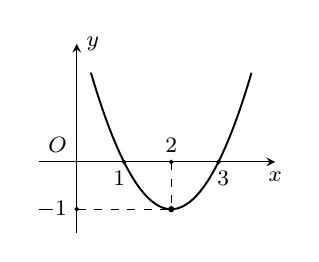
\begin{tikzpicture}[smooth,samples=300,scale=0.6,>=stealth,font=\footnotesize]
			\draw[->] (-0.8,0)--(4.2,0) node[below]{$x$};
			\draw[->] (0,-1.5)--(0,2.5) node[right]{$y$};
			\draw (0,0) node[above left]{$O$};
			\draw[line width=0.7pt,domain=0.3:3.7] plot(\x,{(\x)^2-4*(\x)+3});
			\draw[fill=black] (2,-1) circle(1.5pt) (2,0) circle(1pt) (0,-1) circle(1pt) (1,0) circle(1pt) (3,0) circle(1pt);
			\draw[dashed] (2,0)node[above]{$2$}--(2,-1)--(0,-1)node[left]{$-1$};
			\node[below] at (0.9,0) {$1$};
			\node[below] at (3.1,0) {$3$};
	\end{tikzpicture}}
	\loigiai{
	Vì đồ thị của hàm số $f(x)$ là một parabol nên $f(x)=ax^2+bx+c$ $(a\ne 0)$.\\
	Đồ thị hàm số $f(x)$ đi qua các điểm $(1;0)$, $(2;-1)$, $(3;0)$ nên ta có hệ phương trình
	$$\heva{&a+b+c=0 \\ &4a+2b+c=-1 \\ &9a+3b+c=0}\Leftrightarrow\heva{&a=1 \\ &b=-4 \\ &c=3.}$$
	Do đó $f(x)=x^2-4x+3$.\\
	Vậy $\displaystyle\int\limits_0^3 (x-1)(x^2-4x+3)\mathrm{ \,d}x=\displaystyle\int\limits_0^3(x^3-5x^2+7x-3)\mathrm{ \,d}x=-\dfrac{9}{4}$.
	}
\end{ex}\cham{5}

\begin{ex}%[Thi thử L2, Nguyễn Khuyến, Nam Định, 2018]%[Nguyễn Tài Tuệ, dự án EX10]%[2D3B2-1]%
	Cho hàm số $f(x)=\left\{\begin{aligned}& x & \text {khi } &x\ge 1 \\ &1& \text {khi } &x<1  \end{aligned}\right.$. Tính tích phân $I=\displaystyle\int\limits_0^2 {f(x)\mathrm{\,d}x}$.
	\choice
	{$ I=4 $}
	{\True $ I=\dfrac{5}{2} $}
	{$ I=2 $}
	{$ I=\dfrac{3}{2} $}
	\loigiai{
		Ta có $I=\displaystyle\int\limits_0^2 f(x)\mathrm{\,d}x=\displaystyle\int\limits_{0}^{1}f(x)\mathrm{\,d}x +\displaystyle\int\limits_{1}^{2} f(x)\mathrm{\,d}x=\displaystyle\int\limits_{0}^{1} 1\mathrm{\,d}x+\displaystyle\int\limits_{1}^{2} x \mathrm{\,d}x =\dfrac{5}{2}$.
	}
\end{ex}\cham{3}

\begin{ex}%[2D3B2-1]
	Cho hàm số $y=f(x)=\heva{&3x^2 &\text{khi}\ 0\le x\le 1\\ &4-x &\text{khi}\ 1\le x\le 2}$. Tính tích phân $\displaystyle\int\limits_{0}^{2}f(x)\mathrm{\,d}x$.
	\choice
	{\True $\dfrac{7}{2}$}
	{$1$}
	{$\dfrac{5}{2}$}
	{$\dfrac{3}{2}$}
	\loigiai{
		Ta có
		\begin{align*}
			\displaystyle\int\limits_{0}^{2}f(x)\mathrm{\,d}x=\displaystyle\int\limits_{0}^{1}3x^2\mathrm{\,d}x+\displaystyle\int\limits_{1}^{2}(4-x)\mathrm{\,d}x=\dfrac{7}{2}.
		\end{align*}
	}
\end{ex}\cham{3}

\begin{ex}%[Võ Văn Lê-Phan Tấn Phú]%[Biên Hòa lần 2]%[12-EX-11-2020]%[2D3B2-1]%Câu 8.
	Biết $I=\displaystyle\int\limits_1^5\dfrac{2|x-2|+1}{x}\mathrm d x=4+a\ln 2+b\ln 5$ với $a$, $b$ là các số nguyên. Tính $S=a-b$.
	\choice
	{$S=9$}
	{$S=5$}
	{$S=-3$}
	{\True $S=11$}
	\loigiai{
		Ta có:
		\begin{tikzpicture}[line join=round,line cap=round, font=\footnotesize,scale=1,>=stealth]
			\draw(-1,0)--(5,0);
			\draw(0,-0.7)--(0,0.7);
			\draw(-0.7,0)node[above]{$x$}node[below]{$x-2$}(0.5,0)node[above]{$1$}node[below]{$\big|$}(1.5,0)node[below]{$-$}(2.5,0)node[above]{$2$}node[below]{$0$}(3.5,0)node[below]{$+$}(4.5,0)node[above]{$5$}node[below]{$\big|$};
		\end{tikzpicture}
		\allowdisplaybreaks
		\begin{eqnarray*}
			I&=&\displaystyle\int\limits_1^5 \dfrac{2|x-2|+1}{x}\,\mathrm dx\\
			&=&\int_1^2\dfrac{-2(x-2)+1}{x}\,\mathrm dx+\displaystyle\int\limits_2^5\dfrac{2(x-2)+1}{x}\,\mathrm dx\\
			&=&\left(5\ln |x|-2 x\right)\Big|_1^2+\left(2x-3\ln |x|\right)\Big|_2^5\\
			&=&4+8\ln 2-3\ln 5.
		\end{eqnarray*}
		Vậy $S=a-b=8-(-3)=11$.
	}
\end{ex}\cham{10}
\ind{PHẦN II.} \inden{Câu trắc nghiệm đúng sai. Trong mỗi ý a), b), c), d) ở mỗi câu, học sinh chọn đúng hoặc sai.}\\

\begin{ex}
	Cho $\displaystyle\int_{-3}^0 f(x) \mathrm{d} x=-4$ và $\displaystyle\int_{-3}^0 g(x) \mathrm{d} x=-3$. Xét tính đúng sai của các khẳng định sau:
	\choiceTF
	{\True $\displaystyle\int_{-3}^0[f(x)+g(x)] \mathrm{d} x=-7$}
	{$\displaystyle\int_{-3}^0[f(x)-g(x)] \mathrm{d} x=1$}
	{\True $\displaystyle\int_{-3}^0-3 f(x) \mathrm{d} x=12$}
	{$\displaystyle\int_{-3}^0[2 f(x)+3 g(x)] \mathrm{d} x=-51$}
	\loigiai{
	a) Đúng. $\displaystyle\int_{-3}^0[f(x)+g(x)] \mathrm{d} x=\displaystyle\int_{-3}^{0}f(x)\mathrm{ \,d}x+\displaystyle\int_{-3}^{0}g(x)\mathrm{ \,d}x=-4-3=-7$.\\
	b) Sai. $\displaystyle\int_{-3}^0[f(x)-g(x)] \mathrm{d} x=\displaystyle\int_{-3}^{0}f(x)\mathrm{ \,d}x-\displaystyle\int_{-3}^{0}g(x)\mathrm{ \,d}x=-4+3=-1$.\\
	c) Đúng. $\displaystyle\int_{-3}^{0}-3f(x)\mathrm{ \,d}x=-3\displaystyle\int_{-3}^{0}f(x)\mathrm{ \,d}x=-3\cdot (-4)=12$.\\
	d) Sai. $\displaystyle\int_{-3}^0[2f(x)+3g(x)] \mathrm{d} x=2\displaystyle\int_{-3}^{0}f(x)\mathrm{ \,d}x+3\displaystyle\int_{-3}^{0}g(x)\mathrm{ \,d}x=2\cdot (-4)+3\cdot (-3)=-17$.	
	}
\end{ex}
\cham{12}
\begin{ex}
	Cho hàm số $y=f(x)$ có đạo hàm $f^{\prime}(x)$ liên tục trên $[0 ; 4]$ biết	$\displaystyle\int_0^1 f^{\prime}(x) \mathrm{d} x=-2$; $\displaystyle\int_1^3 f^{\prime}(x) \mathrm{d} x=3$; $\displaystyle\int_3^4 f^{\prime}(x) \mathrm{d} x=-5 \text { và } f(1)=1$. Xét tính đúng sai của các khẳng định sau:
	\choiceTF
	{\True $\displaystyle\int_0^3 f^{\prime}(x) \mathrm{d} x=1$}
	{$\displaystyle\int_1^4 f^{\prime}(x) \mathrm{d} x=2$}
	{$f(0)=-3$}
	{\True $f(4)=-1$}
	\loigiai{	
	a) Đúng. $\displaystyle\int_{0}^3 f'(x) \mathrm{d} x=\displaystyle\int_{0}^{1}f'(x)\mathrm{ \,d}x+\displaystyle\int_{1}^{3}f'(x)\mathrm{ \,d}x=-2+3=1$.\\
	b) Sai. $\displaystyle\int_{1}^4 f'(x) \mathrm{d} x=\displaystyle\int_{1}^{3}f'(x)\mathrm{ \,d}x+\displaystyle\int_{3}^{4} f'(x)\mathrm{ \,d}x=3-5=-2$.\\
	c) Sai. $-2=\displaystyle\int_{0}^{1} f'(x)\mathrm{ \,d}x=f(1)-f(0)\Rightarrow f(0)=f(1)+2=3$.\\
	d) Đúng. $-2=\displaystyle\int_{1}^{4} f'(x)\mathrm{ \,d}x=f(4)-f(1)\Rightarrow f(4)=-2+f(1)=-1$.
	}
\end{ex}
\cham{14}

\begin{ex}
	Cho hàm số $y=f(x)$ thỏa mãn $f^{\prime}(x)=a x+\dfrac{b}{x^2}, f(2)=5, f(1)=4, f^{\prime}(1)=0$. Xét tính đúng sai của các khẳng định sau:
	\choiceTF
	{\True $f^{\prime}(x)=a\left(x-\dfrac{1}{x^2}\right) \forall x \in \mathbb{R} \backslash\{0\}$}
	{$\displaystyle\int_1^2 f^{\prime}(x) \mathrm{d} x=-1$}
	{\True $a=1 ; b=-1$}
	{$f(10)<50$}
	\loigiai{
		\begin{enumerate}[a)]
			\item Đúng. Ta có $f^{\prime}(1)=0 \Leftrightarrow a+b=0 \Leftrightarrow b=-a$. Khi đó:
			$$
			f^{\prime}(x)=a x+\frac{b}{x^2}=a x-\frac{a}{x^2}=a\left(x-\frac{1}{x^2}\right), \forall x \in \mathbb{R} \backslash\{0\}.
			$$
			\item  Sai. $\displaystyle\int_1^2 f'(x) \mathrm{d} x=f(2)-f(1)=5-4=1$.
			\item  Đúng. Ta có
			$$
			f(x)=\displaystyle\int f^{\prime}(x) \mathrm{d} x=a\left(\frac{x^2}{2}+\frac{1}{x}\right)+C
			$$			
			Mà $f(2)=5$ và $f(1)=4$ nên ta có $\heva{& 2,5a+C=5\\&1,5a+C=4}\Leftrightarrow\heva{&a=1\\&C=2,5}$.\\
			Có $a=1$ và $b=-a \Rightarrow b=-1$.
			\item Sai. $f(x)=\dfrac{x^2}{2}+\dfrac{1}{x}+2,5 \Rightarrow f(10)=52,6>50$.
		\end{enumerate}
	}
\end{ex}
\cham{15}
\begin{ex}
	Cho hàm số $f(x)=\left\{\begin{array}{ll}x^2+1 & \text { khi } x>1 \\ -2 x-a & \text { khi } x \leq 1\end{array}\right.$. Biết hàm số $f(x)$ liên tục trên $\mathbb{R}$. Xét tính đúng sai của các khẳng định sau:
	\choiceTF
	{$f(1)=2$}
	{$3 \displaystyle\int_2^4 f(x) \mathrm{\,d} x=62$}
	{$a>0$}
	{$\displaystyle\int_{-1}^4 f(x) \mathrm{\,d} x \geq 29$}
	\loigiai{
		
	}
\end{ex}
\cham{14}
\begin{ex}
	Cho hàm số $f(x)=\dfrac{1}{x^2-7 x+12}$.
	\choiceTF
	{Hàm số xác định trên $\mathbb{R}$}
	{\True Họ nguyên hàm của hàm số $f(x)$ là $\ln |x-4|-\ln |x-3|+C$ với mọi $x \in \mathbb{R} \backslash\{3 ; 4\}$}
	{$\displaystyle\int_0^2 f(x) \mathrm{d} x=\ln 2-\ln 3$}
	{\True Nếu $\displaystyle\int_0^1 f(x) \mathrm{d} x=a \ln 3+b \ln 2$ với $a, b$ là số nguyên thì $a^2-b^2=-5$}
	\loigiai{
	a) Sai. Điều kiện xác định: $x^2-7x+12\ne 0\Leftrightarrow \hoac{x\ne 4\\x\ne 3}$. Vậy tập xác định $D=\mathbb{R}\backslash\left\{3;4\right\}$.\\
	b) Đúng. $\dfrac{1}{x^2-7x+12}=\dfrac{1}{(x-3)(x-4)}=\dfrac{1}{x-4}-\dfrac{1}{x-3}$.\\
	Suy ra: $\displaystyle\int{f(x)}\mathrm{ \,d}x=\displaystyle\int\left(\dfrac{1}{x-4}-\dfrac{1}{x-3}\right)\mathrm{ \,d}x=\ln|x-4|-\ln|x-3|+C$.\\
	c) Sai. $\displaystyle\int_0^2 f(x) \mathrm{d} x=\left(\ln|x-4|-\ln|x-3|\right)\bigg|_{0}^{2}=\ln 2-\ln 4+\ln 3=\ln 3-\ln 2$.\\
	d) Đúng. $\displaystyle\int_0^1 f(x) \mathrm{d} x=\left(\ln|x-4|-\ln|x-3|\right)\bigg|_{0}^{1}=\ln 3 -\ln 2-\ln 4+\ln 3 =2\ln 3-3\ln 2$.\\
	Suy ra: $a=2, b=-3$. Vậy $a^2-b^2=2^2-(-3)^2=-5$.
	}
\end{ex}
\cham{14}
\Closesolutionfile{ans}
\begin{dang}{Bài toán thực tế có sử dụng tích phân}
	\begin{enumerate}[1.]
		\item  Nếu hàm số $f(x)$ có đạo hàm $f^{\prime}(x)$ và $f^{\prime}(x)$ liên tục trên đoạn $[a; b]$ thì
		$$f(b)-f(a)=\displaystyle\int\limits_a^b f^{\prime}(x) \mathrm{\,d}x.$$
		\item Giá trị trung bình của hàm số liên tục $f(x)$ trên đoạn $[a ; b]$ được định nghĩa là
		
		$$
		\dfrac{1}{b-a} \displaystyle\int\limits_{a}^{b} f(x) \mathrm{d} x
		$$
		\item Ta đã biết rằng, đạo hàm của quãng đường di chuyển theo thời gian bằng tốc độ của chuyển động tại mỗi thời điểm $\left(v(t)=s^{\prime}(t)\right)$. Do đó, nếu biết tốc độ $v(t)$ tại mọi thời điểm $t \in[a; b]$ thì tính được quãng đường di chuyển trong khoảng thời gian từ $a$ đến $b$ theo công thức
		$$
		s=s(b)-s(a)=\displaystyle\int\limits_a^b v(t) \mathrm{\,d}t.
		$$
	\end{enumerate}
\end{dang}
\boxmini{BÀI TẬP TỰ LUẬN}
\setcounter{vd}{0}

\begin{vd}
	Lợi nhuận biên của một sản phẩm được mô hình hoá bởi
	
	$$
	P^{\prime}(x)=-0,0005 x+12,2
	$$
	\begin{enumEX}[a)]{1}
		\item Tìm sự thay đổi lợi nhuận khi doanh số bán hàng tăng từ 100 lên 101 đơn vị.
		\item Tìm sự thay đổi lợi nhuận khi doanh số bán hàng tăng từ 100 lên 110 đơn vị.
	\end{enumEX}
	\loigiai{
		\begin{enumerate}[a)]
			\item Sự thay đổi lợi nhuận khi doanh số bán hàng tăng từ 100 lên 101 đơn vị là
			
			$$
			\begin{aligned}
				\displaystyle\int_{100}^{101} P^{\prime}(x) \mathrm{ \,d} x & =\displaystyle\int_{100}^{101}(-0,0005 x+12,2) \mathrm{ \,d} x \\
				& =\left.\left(-0,0005 \cdot \dfrac{x^2}{2}+12,2 x\right)\right|_{100} ^{101}=12,14975 .
			\end{aligned}
			$$
			\item Sự thay đổi lợi nhuận khi doanh số bán hàng tăng từ 100 lên 110 đơn vị là
			
			$$
			\begin{aligned}
				\displaystyle\int_{100}^{110} P^{\prime}(x) \mathrm{d} x & =\displaystyle\int_{100}^{110}(-0,0005 x+12,2) \mathrm{d} x \\
				& =\left.\left(-0,0005 \cdot \dfrac{x^2}{2}+12,2 x\right)\right|_{100} ^{110}=121,475
			\end{aligned}
			$$
	\end{enumerate}}
\end{vd}\dongcham{3}

\begin{vd}
	Giả sử nhiệt độ (tính bằng ${ }^{\circ} \mathrm{C}$ ) tại thời điểm $t$ giờ trong khoảng thời gian từ 6 giờ sáng đến 12 giờ trưa ở một địa phương vào một ngày nào đó được mô hình hoá bởi hàm số
	
	$$
	T(t)=20+1{,}5(t-6), 6 \leq t \leq 12 .
	$$
	Tìm nhiệt độ trung bình vào ngày đó trong khoảng thời gian từ 6 giờ sáng đến 12 giờ trưa.
	\loigiai{
		Nhiệt độ trung bình vào ngày đó trong khoảng thời gian từ 6 giờ sáng đến 12 giờ trưa bằng
		$$\dfrac{1}{12-6}\int_{6}^{12} \left[20+1{,}5\left(t-6\right)\right]\mathrm{\,d}t=\dfrac{49}{2}.$$
	}
\end{vd}\dongcham{3}

\begin{vd}
	Ở nhiệt độ $37^{\circ} \mathrm{C}$, một phản ứng hoá học từ chất đầu $A$, chuyển hoá thành chất sản phẩm $B$ theo phương trình: $A \rightarrow B$. Giả sử $y(x)$ là nồng độ chất $A$ (đơn vị $\mathrm{mol} \mathrm{L}^{-1}$ ) tại thời gian $x$ (giây), $y(x)>0$ với $x \geq 0$, thoả mãn hệ thức: $y^{\prime}(x)=-7.10^{-4} y(x)$ với $x \geq 0$. Biết rằng tại $x=0$, nồng độ (đầu) của $A$ là $0,05 \mathrm{~mol} \mathrm{~L}^{-1}$. 
	\begin{enumEX}[a)]{1}
		\item Xét hàm số $f(x)=\ln y(x)$ với $x \geq 0$. Hãy tính $f^{\prime}(x)$ từ đó tìm hàm số $f(x)$.
		\item Giả sử ta tính nồng độ trung bình chất $A$ (đơn vị $\mathrm{mol} \mathrm{L}^{-1}$ ) từ thời điểm $a$ (giây) đến thời điểm $b$ (giây) với $0<a<b$ theo công thức $\dfrac{1}{b-a} \displaystyle\int_a^b y(x) \mathrm{\,d} x$.	Xác định nồng độ trung bình của chất $A$ từ thời điểm 15 giây đến thời điểm 30 giây.
	\end{enumEX}
	\loigiai{
		\begin{enumerate}[a)]
			\item Ta có $f(x)=\ln y(x) \Rightarrow f^{\prime}(x)=\frac{y^{\prime}(x)}{y(x)}=-7.10^{-4} \Rightarrow f(x)=-7.10^{-4} x$.
			\item $f(x)=-7.10^{-4} x \Rightarrow \ln y(x)=-7.10^{-4} x \Leftrightarrow y(x)=e^{-7.10^{-4} x}$.	Nồng độ trung bình của chất A từ thời điểm 15 giây đến thời điểm 30 giây là:
			$$\frac{1}{30-15} \displaystyle\int_{15}^{30} y(x) \mathrm{d} x=\frac{1}{15} \displaystyle\int_{15}^{30} e^{-7 \cdot 10^{-4} x} \mathrm{~d} x=\left.\frac{1}{15} \frac{e^{-7 \cdot 10^{-4}x}}{-7 \cdot 10^{-4}}\right|_{15} ^{30}=0,98\left(L^{-1}\right)$$
		\end{enumerate}
		
	}
\end{vd}
\dongcham{10}
\begin{vd}
	Người ta ước tính rằng, sau $t$ năm kể từ bây giờ, cộng đồng dân cư ở ven hồ nước sẽ thay đổi với tốc độ $v(t)=0,6t^2+0,2t+5$ nghìn người mỗi năm. Các nhà môi trường học thấy rằng mức độ ô nhiễm trong hồ tăng với tốc độ xấp xỉ 5 đơn vị mỗi 1000 người. Hỏi mức độ ô nhiễm trong hồ tăng lên bao nhiêu đơn vị trong hai năm tới?
	\loigiai{
		Số người tăng lên sau 2 năm $ \displaystyle\int \limits_{0}^{2} v(t) \mathrm{d}t=\displaystyle\int \limits_{0}^{2} \left( 0,6t^2+0,2t+5\right)  \mathrm{d}t=12$ (nghìn người).\\
		Khi đó, mức độ ô nhiễm tăng lên là $12 \times 5 = 60$ (đơn vị).
		
	}
\end{vd}
\dongcham{5}
\begin{vd}
	Một chiếc ô tô đang chạy với vận tốc $ 15 $ m/s thì người lái xe hãm phanh. Sau khi hãm phanh, ô tô chuyển động chậm dần đều với vận tốc $ v(t)=-3t+15 $ m/s, trong đó $ t $ (giây). Hỏi từ lúc hãm phanh đến khi dừng hẳn, ô tô di chuyển được bao nhiêu mét?
	\loigiai{
		Khi xe dừng hẳn thì $ v(t)=0 $ hay là $ -3t+15=0 \Leftrightarrow t=5$.\\
		Khi đó, quãng đường $ s $ xe đi được tính từ lúc bắt đầu hãm phanh đến khi dừng hẳn là
		$$ \displaystyle\int \limits_{0}^{5} (-3t+15) \mathrm{d}t=\left. \left(-\dfrac{3t^2}{2}+15t\right)\right |_0^5=37{,}5.$$
	}
\end{vd}\dongcham{5}

\begin{vd}
	\immini{Hình bên là đồ thị vận tốc $v(t)$ của một vật $(t=0$ là thời điểm vật bắt đầu chuyển động).
		\begin{enumerate}
			\item Viết công thức của hàm số $v(t)$ với $t \in[0 ; 6]$.
			\item Tính quãng đường vật di chuyển được trong $6$ giây đầu  tiên.
	\end{enumerate}}{	\begin{tikzpicture}[scale=0.8,>=stealth, font=\footnotesize, line join=round, line cap=round]
			\def\xmin{-1.0} \def\xmax{7.5}
			\def\ymin{-1} \def\ymax{4}
			\draw[->] (\xmin,0)--(\xmax,0) node [below]{$t(\text{s})$};
			\draw[->] (0,\ymin)--(0,\ymax) node [above]{$v(\text{m/s})$};
			\draw (0,0)--(2,3)--(6,3);
			\draw[dashed](2,0)--(2,3)--(0,3) (6,0)--(6,3);
			%\fill (0,0) circle(1pt)[above left]{$O$};
			\fill (0,3) circle(1.0pt)node[left]{$3$}
			(2,0) circle(1.0pt)node[below]{$2$}
			(6,0) circle(1.0pt)node[below]{$6$}
			(6,3) circle(1.0pt)
			(2,3) circle(1.0pt); \fill (0,0) circle(1.0pt)node[above left]{$O$};
	\end{tikzpicture}}
	\loigiai{
		\begin{enumerate}
			\item 	
			Từ đồ thị ta thấy $v(t)=\heva{&\dfrac{3}{2}t\;\text{nếu}\;t\le2\\& 3 \;\text{nếu}\; 2<t\le 6}.$ 
			
			\item Quãngđường vật đi được trong $2$ giây đầu tiên là
			$$L_1=\displaystyle\int\limits_{0}^2 \dfrac{3}{2}t \mathrm{d} t=\dfrac{3}{4}t^2\bigg|_0^2=3\;\text{m}.$$
			Quãng đường vật đi được từ giây thứ $2$ đến giây thứ $6$ là
			$$L_2=\displaystyle\int\limits_{2}^{6} 3\mathrm{ \,d}t=12\;\text{m}.$$
			Vậy quãng đường vật đi được trong $6$ giây đầu tiên là $3+12=15$ m.
		\end{enumerate}
	}
\end{vd}\dongcham{14}

\boxmini{BÀI TẬP TRẮC NGHIỆM}
\setcounter{ex}{0}
\Opensolutionfile{ans}[ans/2D4-B2-d3]

\begin{ex}
	Một vật chuyển động theo phương trình $v=10t+5\; \mathrm{m/s}$. Tính quãng đường vật đi được kể từ thời điểm $t=0$ (giây) đến thời điểm $t=3$ (giây).
	\choice
	{\True $60$ m}
	{$15$ m}
	{$30$ m}
	{$50$ m}
	\loigiai{
		Quãng đường $s$ vật đi được từ thời điểm $t=0$ (giây) đến thời điểm $t=3$ (giây) bằng
		$$s=\displaystyle \int \limits_0^3 \left(10t+5\right) \mathrm{\, d}t=\left.\left(5t^2+5t\right)\right|_0^3=60\; \text{m}.$$
	}
\end{ex}\cham{3}

\begin{ex}%[2D3B3-7]%[Hải Phòng, 2018]%[Phan Anh Tiến, 12-EX-05]%
	Một vật chuyển động chậm dần đều với vận tốc $v(t)=180-20t$ (m/s). Tính quãng đường mà vật di chuyển từ thời điểm $t=0$ đến lúc vật dừng lại.
	\choice
	{$ 180 $ m}
	{$ 9$ m}
	{$ 160 $ m}
	{\True $ 810 $ m}
	\loigiai{
		Thời điểm vật dừng lại thì $v(t)=0\Leftrightarrow t=9$.\\
		Quãng đường vật di chuyển là $\displaystyle\int\limits_0^9(180-20t)\mathrm{\,d}t=\left( 180t-10t^2\right) \bigg| _0^9=810$.
	}
\end{ex}\cham{3}

\begin{ex}%[THPT 19-5 Kim Bôi, lần 1, 2018 - 2019]%[Đỗ Viết Lân, Ex7 2019]%[2D3K3-7]%
	Một ô tô chuyển động nhanh dần đều với vận tốc $v(t) = 7t$ (m/s). Đi được $5$ (s) người lái xe phát hiện chướng ngại vật và phanh gấp, ô tô tiếp tục chuyển động chậm dần đều với gia tốc $a = -35$ (m/s$^2$). Tính quãng đường của ô tô đi được từ lúc bắt đầu chuyển bánh cho đến khi dừng hẳn.
	\choice
	{$96{,}5$ mét}
	{\True $105$ mét}
	{$87{,}5$ mét}
	{$102{,}5$ mét}
	\loigiai{
		Quãng đường đi được trong $5$ giây đầu là $s_1=\displaystyle\int\limits_0^5 7t\mathrm{d}t=7\left.\dfrac{t^2}{2}\right|_0^5=87{,}5$ mét.\\
		Vận tốc của chuyển động sau khi phanh là: $v_2(t)=-35t+C$ (m/s). Vì $v_2(0)=35$ nên suy ra $C=35$. Vậy $v_2(t)=35-35t$ (m/s).\\
		Khi xe dừng hẳn thì $35-35t=0 \Leftrightarrow t = 1$.\\
		Quãng đường ô tô đi được từ khi phanh đến khi dừng lại hẳn là $$s_2=\displaystyle\displaystyle\int\limits_0^1 (35 - 35t)\mathrm{d}t=\left.\left(35t - 35\dfrac{t^2}{2}\right)\right|_0^1=17{,}5.$$
		Vậy tổng quãng đường là $105$ mét.
	}
\end{ex}\cham{4}

\begin{ex}
	Một vật chuyển động với gia tốc $a(t)=-20(1+2 t)^{-2}\left(\mathrm{~m} / \mathrm{s}^2\right)$. Khi $t=0$ thì vận tốc của vật là $30(\mathrm{~m} / \mathrm{s})$. Tính quãng đường vật đó đi chuyển sau 2 giây ( $m$ là mét, $s$ là giây, kết quả làm tròn đến hàng đơn vị).
	\choice
	{46 m}
	{\True 48 m}
	{47 m}
	{49 m}
	\loigiai{
		$v(t)=\displaystyle\int a(t)\mathrm{\,d}t=10(1+2t)^{-1}+C$\\
		Với $v(0)=30 \Rightarrow C=20$. Vậy $v(t)=10(1+2t)^{-1}+20$.\\
		Tính quãng đường vật đó đi chuyển sau 2 giây là
		$$v(t)=\displaystyle\int\limits_0^2 10(1+2t)^{-1}+20\mathrm{\,d}t\approx 48 \,m$$
	}
\end{ex}
\cham{4}
\begin{ex}
	Một ô tô đang chạy với vận tốc $20$ (m/s) thì người lái xe phát hiện có hàng rào chắn ngang đường ở phía trước cách xe $45$ m (tính từ đầu xe tới hàng rào) nên người lái đạp phanh. Từ thời điểm đó, xe chuyển động chậm dần đều với vận tốc $v(t)=-5t+20$ (m/s), $t$ là thời gian được tính từ lúc người lái đạp phanh. Hỏi khi xe dừng hẳn, khoảng cách từ xe đến hàng rào là bao nhiêu mét?
	\choice
	{$3$}
	{$4$}
	{$6$}
	{\True $5$}
	\loigiai
	{Xe dừng lại khi $v(t)=0\Leftrightarrow -5t+20=0\Leftrightarrow t=4$ (s).\\
		Quãng đường ô tô đi được từ lúc bắt đầu phanh đến khi xe dừng lại là\\
		$s=\displaystyle\int\limits_0^4 v(t)\mathrm{\,d}t =\displaystyle\int\limits_0^4 (-5t+20)\mathrm{\,d}t =\left(-\dfrac{5}{2}t^2+20t\right)\bigg|_0^4=-40+80=40$ (m).\\
		Vậy khi xe dừng hẳn, khoảng cách từ xe đến hàng rào là $45-40=5$ (m).}
\end{ex}\cham{4}

\begin{ex}
	Để đảm bảo an toàn khi lưu thông trên đường, các xe ô tô khi dừng đèn đỏ phải cách nhau tối thiểu 1 m . Một ô tô $A$ đang chạy với vận tốc $16 \mathrm{~m} / \mathrm{s}$ bỗng gặp ô tô $B$ đang dừng đèn đỏ nên ô tô $A$ hãm phanh và chuyển động chậm dần đều với vận tốc được biểu thị bởi công thức $v_A(t)=16-4 t$ (đơn vị tính bằng $\mathrm{m} / \mathrm{s}$ ), thời gian tính bằng giây. Hỏi rằng để có 2 ô tô $A$ và $B$ đạt khoảng cách an toàn khi dừng lại thì ô tô $A$ phải hãm phanh khi cách ô tô $B$ một khoảng ít nhất là bao nhiêu mét?	
	\choice
	{33 m}
	{12 m}
	{31 m}
	{32 m}
	\loigiai{
		Ta có: $v_A(0)=16 \mathrm{~m} / \mathrm{s}$.\\
		Khi xe $A$ dừng hẳn: $v_A(t)=0 \Leftrightarrow t=4 \mathrm{~s}$.\\
		Quãng đường từ lúc xe $A$ hãm phanh đến lúc dừng hẳn là $s=\int_0^4(16-4 t) \mathrm{d} t=32 \mathrm{~m}$.\\
		Do các xe phải cách nhau tối thiểu 1 m để đảm bảo an toàn nên khi dừng lại ô tô $A$ phải hãm phanh khi cách ô tô $B$ một khoảng ít nhất là 33 m .	
	}
\end{ex}
\cham{7}
\begin{ex}
	Một nhà nghiên cứu ước tính rằng sau $t$ giờ kể từ $0$ giờ đêm, nhiệt độ tại địa phương X được cho bởi hàm số $C(t)=40-\dfrac{2}{3}\left(1-10 \right)^2$ ($^\circ C$), với $0 \le t <24$. Hỏi nhiệt độ trung bình của địa phương X từ 8 giờ sáng đến 5 giờ chiều là bao nhiêu? (\textit{kết quả làm tròn đến hàng phần trăm})
	\choice
	{$32,87^\circ C$}
	{\True $31,33^\circ C$}
	{$27,42^\circ C$}
	{$29,37^\circ C$}
	\loigiai{
		Nhiệt độ trung bình trong khoảng thời gian từ 8 giờ sáng đến 17 giờ chiều là
		
		$$
		T=\frac{1}{17-8} \int_8^{17}\left[40-\frac{2}{3}(t-10)^2\right] \mathrm{ \,d} t=\dfrac{94}{3} \approx 31,33\left({ }^{\circ} \mathrm{C}\right)
		$$
	}
\end{ex}
\cham{8}
\begin{ex}
	Ở nhiệt độ $37^{\circ} \mathrm{C}$, một phản ứng hóa học từ chất A , chuyển hóa thành sản phẩm chất B theo phương trình: $\mathrm{A} \rightarrow \mathrm{B}$. Giả sử $f(x)$ là nồng độ chất A (đơn vi mol/L) tại thời gian $x$ giây được cho bởi hàm $f(x)=e^{-7.10^{-4} x}$ với $x \geq 0$. Xác định nồng độ trung bình của chất A từ thời điểm 15 giây đến thời điểm 30 giây (\textit{kết quả làm tròn đến hàng phần trăm}).
	\choice
	{$0,92$ mol/L}
	{$0,72$ mol/L}
	{$0,78$ mol/L}
	{\True $0,98$ mol/L}
	\loigiai{
		Nồng độ trung bình của chất A từ thời điểm 15 giây đến thời điểm 30 giây là
		
		$$
		\frac{1}{30-15} \int_{15}^{30} f(x) \mathrm{d} x=\frac{1}{15} \int_{15}^{30} e^{-7.10^{-4} x} \mathrm{~d} x=0,98
		$$
	}
\end{ex}
\cham{8}
\begin{ex}%[2D3T2-1]
	Tốc độ $v~(\mathrm{m}/s)$ của một thang máy di chuyển từ tầng 1 lên tầng cao nhất theo thời gian $t$ (giây) được cho bởi công thức:
	$$v(t)=\heva{&t,\quad\quad\quad\quad 0 \leq t \leq 2, \\
		&2, \quad\quad\quad\quad 2<t \leq 20, \\
		&12-0{,}5t,\; 20<t \leq 24.}$$
	Tính tốc độ trung bình của thang máy.
	\choice
	{$1{,}8 \,(\mathrm{m/s})$}
	{$1{,}75 \,(\mathrm{m/s})$}
	{$1{,}5 \,(\mathrm{m/s})$}
	{$1{,}65 \,(\mathrm{m/s})$}
	\loigiai{
		\begin{itemize}
			\item Quãng đường chuyển động của thang máy là
			$$
			\displaystyle\int\limits_0^{24} v(t) \mathrm{\,dt} =\displaystyle\int\limits_0^2 t \mathrm{\,dt}+\displaystyle\int\limits_2^{20} 2 \mathrm{\,dt}+\displaystyle\int\limits_{20}^{24} (12-0{,}5t) \mathrm{\,dt}=42 \,(\mathrm{m}).
			$$
			\item Tốc độ trung bình của thang máy là
			$$\dfrac{1}{24-0} \displaystyle\int\limits_0^{24} v(t) \mathrm{\,d} t=\dfrac{42}{24}=1{,}75 \,(\mathrm{m/s}).$$
		\end{itemize}
		
	}
\end{ex}\cham{8}

\begin{ex}
	Việc thở là những vòng tuần hoàn, mỗi vòng tính từ lúc bắt đầu hít vào đến lúc kết thúc thở ra, thường kéo dài trong 5 s . Vận tốc cực đại của khí là $V(l / s)$ nên vì thế nó được mô hình hoá bởi công thức $v(t)=V \sin \dfrac{3 \pi t}{5}$. Tính thể tích khí hít vào phổi sau thời gian 2 s .
	\choice
	{$1,02V$ (lít)}
	{$1,09V$ (lít)}
	{$1,04V$ (lít)}
	{\True $0,96V$ (lít)}
	\loigiai{
		Vận tốc của khí hít vào được mô hình bởi công thức $v(t)=V \sin \frac{3 \pi t}{5}$.
		Suy ra lượng khí hít vào sau 2 giây là:
		
		$$
		N(2)=\int_0^2 v(x) d x=\int_0^2 V \sin \frac{3 \pi t}{5} d t=\frac{5 V}{3 \pi}\left(1-\cos \frac{3 \pi \cdot 2}{5}\right)=0,96 V
		$$	
	}
\end{ex}
\cham{7}
\begin{ex}
	Khi nghiên cứu một quần thể vi khuẩn, người ta nhận thấy quần thể vi khuẩn đó ở ngày thứ $t$ có số lượng $N(t)$ con. Biết rằng tốc độ phát triển của quần thể đó là $N^{\prime}(t)=\dfrac{8000}{t}$ và sau ngày thứ nhất $(t=1)$ có 250000 con. Sau 6 ngày $(t=6)$, số lượng của quần thể vi khuẩn là
	\choice
	{353584 con}
	{234167 con}
	{288959 con}
	{\True 264334 con}
	\loigiai{
		Ta có $N(6)-N(1)=\displaystyle\int\limits_1^{6} N'(t) \mathrm{\,dt}\Rightarrow N(6)=\displaystyle\int\limits_1^{6} \frac{8000}{t} \mathrm{\,dt}+250000=264334$ (con).
	}
\end{ex}\cham{7}

\begin{ex}
	Cường độ dòng điện (đơn vị: A ) trong một dây dẫn tại thời điểm $t$ giây là: $I(t)=Q^{\prime}(t)=3 t^2-6 t+5$. Với $Q(t)$ là điện lượng (đơn vị: C) truyền trong dây dẫn tại thời điểm $t$. Biết khi $t=1$ giây thì điện lượng truyền trong dây dẫn là $Q(1)=4$. Tính điện lượng truyền trong dây dẫn khi $t=3$.
	\choice
	{$12$C}
	{$14$C}
	{\True $16$C}
	{$7$C}
	\loigiai{
		Ta có $\displaystyle\int_1^3\left(3 x^2-6 x+5\right) \mathrm{\,d} x=Q(3)-Q(1)\Rightarrow Q(3)=\displaystyle\int_1^3\left(3 x^2-6 x+5\right) \mathrm{d} x+Q(1)=12+4=16$C.
	}
\end{ex}
\cham{5}
\begin{ex}
	\immini[thm]{
		Một vật chuyển động trong $4$ giờ với vận tốc $v$(km/h) phụ thuộc thời gian $t$(h) có đồ thị là một phần của đường parabol có đỉnh $I(1;1)$ và trục đối xứng song song với trục tung như hình bên. Tính quãng đường $s$ mà vật đi được trong $4$ giờ kể từ lúc xuất phát.
		\haicot
		{$s=\dfrac{46}{3}$(km)}
		{\True $s=\dfrac{40}{3}$(km)}
		{$s=8$(km)}
		{$s=6$(km)}
	}{
		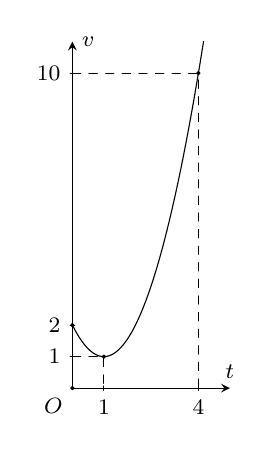
\begin{tikzpicture}[scale=0.4, font=\footnotesize, line join=round, line cap=round, >=stealth]
			\draw[->] (0,0)--(5,0) node[above]{\footnotesize $t$};
			\draw[->] (0,0)--(0,11) node[right] {\footnotesize $v$};
			\foreach \x in {1,4}\draw[shift={(\x,0)},color=black] (0pt,2pt) -- (0pt,-2pt) node[below] {\footnotesize $\x$};
			\foreach \y in {1,2,10}\draw[shift={(0,\y)},color=black] (2pt,0pt) -- (-2pt,0pt) node[left] {$\y$};
			\filldraw (0,0) circle(1.5pt) node [below left] {\footnotesize $O$};
			\filldraw (1,1)circle(1.5pt) (0,2)circle(1.5pt) (4,10)circle(1.5pt);
			\begin{scope}
				\clip (0,0) rectangle (5,11);
				\draw[samples=100,smooth,domain=0:5,variable=\x] plot (\x,{(\x)^2-2*(\x)+2});
			\end{scope}
			\draw[dashed] (0,1)--(1,1)--(1,0);
			\draw[dashed] (0,10)--(4,10)--(4,0);
		\end{tikzpicture}
	}
	\loigiai{
		Vì đồ thị của hàm số $v(t)$ có dạng là một phần của parabol nên $v(t)=at^2+bt+c$ $(a\ne 0,t\ge 0)$.\\
		Đồ thị hàm số $v(t)$ đi qua các điểm $(0;2)$, $(1;1)$, $(4;10)$ nên ta có hệ phương trình
		$$\heva{&c=2 \\ &a+b+c=1 \\ &16a+4b+c=10}\Leftrightarrow\heva{&a=1 \\ &b=-2 \\ &c=2.}$$
		Do đó $v(t)=t^2-2t+2$.\\
		Vậy quãng đường mà vật đi được là $s=\displaystyle\int\limits_0^4 v(t)\mathrm{\,d}t=\int\limits_0^4 (t^2-2t+2)\mathrm{\,d}t=\dfrac{40}{3}$(km).
	}
\end{ex}\cham{5}

\begin{ex}%[Võ Văn Lê]%[TeX - LVĐ - Đợt 3]%[2D3K3-7]%Câu 29
	\immini[thm]{Một vật chuyển động trong $4$ giờ với vận tốc $v$ (km/h) phụ thuộc vào thời gian $t$ (h) có đồ thị như hình bên. Trong khoảng thời gian $3$ giờ kể từ lúc bắt đầu chuyển động đồ thị đó là một phần của đường parabol có đỉnh là $I(2;9)$ với trục đối xứng song song với trục tung, khoảng thời gian còn lại đồ thị là một đoạn thẳng song song với trục hoành. Tính quãng đường $s$ mà vật di chuyển được trong $4$ giờ đó.
		\choice
		{$26{,}5$ km}
		{$24$ km}
		{$28{,}5$ km}
		{\True $27$ km}
	}{
		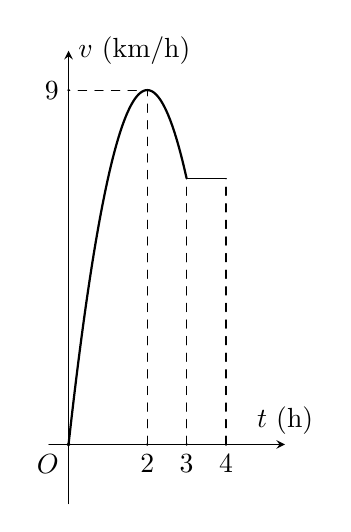
\begin{tikzpicture}[scale=0.5, line join=round, line cap=round,>=stealth]
			\draw [->] (-0.5,0)--(5.5,0) node[above]{$t$ (h)};
			\draw [->] (0,-1.5)--(0,10) node[right]{$v$ (km/h)} ;
			\draw (0,0) node[below left]{$O$} circle(1pt);
			\draw (3,27/4)--(4,27/4);
			\draw [smooth,domain=0:3, samples=300, thick] plot(\x,{(-9/4)*(\x)^2+9*\x});
			\draw[dashed] (2,0)|-(0,9)(3,0)--(3,27/4)(4,0)--(4,27/4);
			\fill (2,0)circle(1pt)node[below]{$2$}(3,0)circle(1pt)node[below]{$3$}(4,0)circle(1pt)node[below]{$4$}(0,9)circle(1pt)node[left]{$9$};
		\end{tikzpicture}
	}
	\loigiai{
		Phương trình parabol có dạng $(P)\colon v=at^2+bt+c$.\\
		$O(0,0)\in (P)\Rightarrow c=0$.\\
		Đỉnh $I(2;9)\in (P)\Rightarrow\hoac{&9=4a+2b\\&2=-\dfrac{b}{2a}}\Leftrightarrow \hoac{&a=-\dfrac{9}{4}\\&b=9.}$\\
		$(P)\colon v=-\dfrac{9}{4}t^2+9t$. Với $t=3\Rightarrow v=\dfrac{27}{4}$\\
		$S=S_1+S_2=\displaystyle\int\limits_0^3\left(-\dfrac{9}{4}t^2+9t\right)\,\mathrm dt+\dfrac{27}{4}\cdot(4-3)=\dfrac{81}{4}+\dfrac{27}{4}=27$ km.
	}
\end{ex}
\cham{6}
\Closesolutionfile{ans}
\ind{PHẦN II.} \inden{Câu trắc nghiệm đúng sai. Trong mỗi ý a), b), c), d) ở mỗi câu, học sinh chọn đúng hoặc sai.}\\
\Opensolutionfile{ans}[ans/2D4-B1-d3-2]

\begin{ex}
	\immini{Một vật chuyển động với vận tốc $v(t)$ được cho bởi hình vẽ:
		\choiceTF
		{\True Vận tốc của vật tại thời điểm $t=3\,(\mathrm{s})$ là 1}
		{\True Vật dừng lại tại $t=4\,(\mathrm{s})$}
		{Quãng đường vật đi được từ lúc $t=1\,(\mathrm{s})$ đến $t=3\,(\mathrm{s})$ là 1 m}
		{\True Quãng đường vật đi được từ $t=0\,(\mathrm{s})$ cho đến khi vật dừng lại là 3 m}
	}{
		\begin{tikzpicture}[smooth,samples=300,scale=1.2,>=stealth]
			\draw[->] (-0.8,0)--(5,0) node [below]{$t(\text{s})$} ;
			\draw[->] (0,-.5)--(0,2) node [above]{$v(\text{m/s})$};
			\draw (0,0) node[above left]{$O$};
			\draw[fill=black] (1,1) circle(1pt) (3,1) circle(1pt) (4,0) circle(1pt);
			\draw (0,0)--(1,1)--(3,1)--(4,0)node[below]{$4$};
			\draw[dashed] (1,0)node[below]{$1$}--(1,1)--(0,1)node[left]{$1$} (3,0)node[below]{$3$}--(3,1);
	\end{tikzpicture}}
	\loigiai{
		\begin{enumerate}[a)]
			\item Đúng. Dựa vào đồ thị ta có $v(3)=1$ vậy vận tốc của vật tại $t=3(\mathrm{~s})$ là $1(\mathrm{~m} / \mathrm{s})$.
			\item Đúng. Ta có: $v(4)=0$ nên vật dừng lại tại $t=4$ (s).
			\item Sai. Quãng đường vật đi được từ lúc $t=1$ đến $t=3$ là: $\displaystyle\int_{1}^{3}\mathrm{ \,d}t=2$. Vậy $S=2$ (m).
			\item Đúng.\\
			Phương trình vận tốc từ $t=0$ đến $t=1$ là: $v(t)=t$.\\
			Phương trình vận tốc từ $t=3$ đến $t=4$ là: $v(t)=-t+4$.\\
			Quãng đường vật đi được từ $t=0$ đến khi dừng lại là: 
			$$S=\displaystyle\int_{0}^{1} t\mathrm{ \,d}t+\displaystyle\int_{1}^{3} \mathrm{ \,d}t+\displaystyle\int_{3}^{4} (-t+4)\mathrm{ \,d}t=3.$$
		\end{enumerate}
	}
\end{ex}
\cham{6}
\begin{ex}
	Một chất điểm chuyển động thẳng trong 19 giây với vận tốc $v(t)$ (đơn vị m/s) là hàm số phụ thuộc vào thời gian $t$ (đơn vị giây) có đồ thị như hình vẽ.
	\begin{center}
		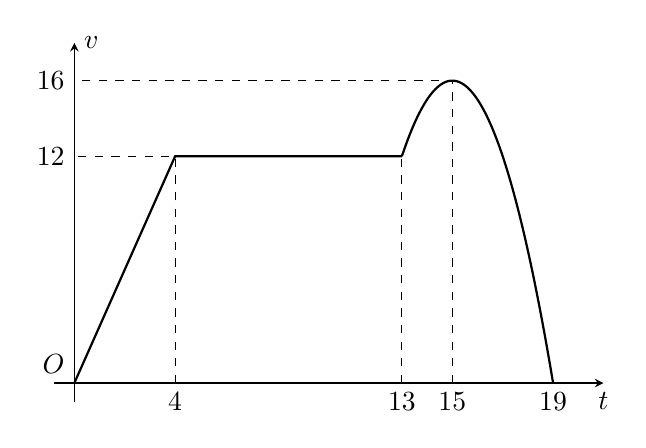
\begin{tikzpicture}[smooth,samples=300,scale=0.8,>=stealth,x=0.4cm,y=0.3cm]
			\draw[->] (-0.8,0)--(21,0) node[below]{$t$};
			\draw[->] (0,-1)--(0,18) node[right]{$v$};
			\draw (0,0) node[above left]{$O$};
			\draw[thick] (0,0)--(4,12)--(13,12);
			\draw[domain=13:19,thick] plot(\x,{-(\x)^2+30*(\x)-209});
			\draw[dashed] (4,0)node[below]{$4$}--(4,12)--(0,12)node[left]{$12$} (13,0)node[below]{$13$}--(13,12) (15,0)node[below]{$15$}--(15,16)--(0,16)node[left]{$16$};
			\node[below] at (19,0) {$19$};
		\end{tikzpicture}
	\end{center}
	\choiceTF
	{Tại thời điểm $t=19$ giây, vận tốc của chất điểm bằng $16 \mathrm{~m} / \mathrm{s}$}
	{\True Quãng đường chất điểm đi được trong khoảng thời gian từ 0 giây đến 4 giây bằng 24 m}
	{\True Trong khoảng thời gian từ 13 giây đến 19 giây, đồ thị của $v(t)$ là một phần của đường parabol. Khi đó $v(t)=-t^2+30 t-209(\mathrm{~m} / \mathrm{s})$}
	{\True Quãng đường chất điểm đi được từ lúc xuất phát đến khi dừng lại bằng 204 m}
	\loigiai{
	a) Sai. Ta có: $v(19)=0$ nên tại thời điểm $t=19$ giây, vận tốc của chất điểm bằng $0$ m/s (tức là vật đứng yên).\\
	b) Đúng. Phương trình vận tốc từ $t=0$ đến $t=4$ là: $v(t)=3t$.\\
	Khi đó quãng đường chất điểm đi được trong khoảng từ 0 giây đến 4 giây là: $\displaystyle\int_{0}^{4} 3t\mathrm{ \,d}t=24$ (m).\\
	c) Đúng. Phương trình vận tốc từ $t=13$ đến $t=19$ là đường parabol có dạng: $y=v(t)=at^2+bt+c$ đi qua ba điểm $(13;12), (15;16), (19;0)$. Ta có hệ phương trình:
	$$\heva{&169a+13b+c=12\\&225a+15b+c=16\\&361a+19b+c=0}\Leftrightarrow\heva{&a=-1\\&b=30\\&c=-209}$$
	Vậy $v(t)=-t^2+30t-209$ (m/s).\\
	d) Đúng. Quãng đường chất điểm đi được từ lúc xuất phát đến khi dừng lại là: $$S=\displaystyle\int_{0}^{4} 3t\mathrm{ \,d}t+\displaystyle\int_{4}^{13} 12\mathrm{ \,d}t+\displaystyle\int_{13}^{19}(-t^2+30t-209)\mathrm{ \,d}t=204 \text{ (m)}.$$
	}
\end{ex}
\cham{8}
\begin{ex}
	Một chất điểm $A$ xuất phát từ $O$, chuyển động thẳng với vận tốc biến thiên theo thời gian bởi quy luật $v(t)=\dfrac{1}{100}t^2+\dfrac{13}{30}t$ (m/s), trong đó $t$ (giây) là khoảng thời gian tính từ lúc $A$ bắt đầu chuyển động. Từ trạng thái nghỉ, một chất điểm $B$ cũng xuất phát từ $O$, chuyển động thẳng cùng hướng với $A$ nhưng chậm hơn $10$ giây so với $A$ và có gia tốc bằng $a$ (m/{s}$^2$) ($a$ là hằng số). Sau khi $B$ xuất phát được $15$ giây thì đuổi kịp $A$. 
	\choiceTF
	{\True Khi chất điểm $B$ bắt đầu xuất phát thì chất điểm $A$ đã đi được $25$ mét}
	{Chất điểm $A$ đi được 15 giây thì bị chất điểm $B$ đuổi kịp}
	{\True Khi chất điểm $B$ đuổi kịp $A$ thì chất điểm $A$ đã đi được $187,5$ mét}
	{\True Vận tốc của $B$ tại thời điểm đuổi kịp $A$ bằng $25$ (m/s)}
	\loigiai{
		a) Đúng. Quãng đường $A$ đi được từ $t=0$ đến $t=10$ là: $\displaystyle\int_{0}^{10} v(t)\mathrm{ \,d}t=25$ (m).\\
		b) Sai. $B$ xuất phát được 15 giây thì đuổi kịp $A$, lúc này $A$ đã đi được $10+15=25$ giây.\\
		c) Đúng. Quãng đường chất điểm $A$ đi được trong $25$ giây là \\
		$$S_A=\displaystyle\displaystyle\int\limits_0^{25} \left(\dfrac{1}{100}t^2+\dfrac{13}{30}t \right) \mathrm{d}t=\left(\dfrac{1}{300}t^3+\dfrac{13}{60}t^2\right) \bigg|_0^{25} =\dfrac{375}{2}=187,5$$
		d) Đúng. Ta có $v_B(t)=\displaystyle\displaystyle\int a \mathrm{\,d}t=at+C$. Do $v_B(0)=0 $ nên $ C=0 \Rightarrow v_B(t)=at$. \\
		Quãng đường chất điểm $B$ đi được trong $15$ giây là \\
		$$S_B=\displaystyle\displaystyle\int\limits_0^{15} at \mathrm{\,d}t=\dfrac{at^2}{2} \bigg|_0^{15} =\dfrac{225a}{2}.$$
		Ta có: $\dfrac{375}{2}=\dfrac{225a}{2} \Leftrightarrow a=\dfrac{5}{3}$. \\
		Vận tốc của $B$ tại thời điểm đuổi kịp $A$ là $v_B(15)=\dfrac{5}{3}\cdot 15=25$ (m/s).}
\end{ex}
\cham{10}
\begin{ex}
	Một người điều khiển ô tô đang ở đường dẫn muốn nhập làn vào đường cao tốc. Khi ô tô cách điểm nhập làn $200$ m, tốc độ của ô tô là $36$ km/h. Hai giây sau đó, ô tô bắt đầu tăng tốc với tốc độ $v(t) = at + b$ ($a$, $b \in \mathbb{R}$, $a > 0$), trong đó $t$ là thời gian tính bằng giây kể từ khi bắt đầu tăng tốc. Biết rằng ô tô nhập làn cao tốc sau $12$ giây và duy trì sự tăng tốc trong $24$ giây kể từ khi bắt đầu tăng tốc.
	\choiceTF
	{\True Quãng đường ô tô đi được từ khi bắt đầu tăng tốc đến khi nhập làn là $180$ m}
	{\True Giá trị của $b$ là $10$}
	{Quãng đường $S(t)$ (đơn vị: mét) mà ô tô đi được trong thời gian $t$ giây ($0 \leq t \leq 24$) kể từ khi tăng tốc được tính theo công thức $S(t) =\displaystyle \int_0^{24} v(t) \mathrm{\,d}t$}
	{Sau $24$ giây kể từ khi tăng tốc, tốc độ của ô tô không vượt quá tốc độ tối đa cho phép là $100$ km/h}
	\loigiai{
		\begin{center}
			\begin{tikzpicture}[line join = round, line cap=round,>=stealth,font=\footnotesize,scale=1]
				\draw 
				(0,0)node[above]{$A$} node[yshift=25pt,pos=0.5]{$v_0=36$ km/h}
				-- (3,0)node[above]{$B$} node[yshift=-10pt,pos=0.5]{$2$ giây} 
				node[xshift=20pt,yshift=25pt]{$v(t)=at+b$ (m/s)}--(8,0) node[above]{$C$}--(14,0) node[above]{$D$}
				;
				\draw[<->] (3,-0.75)--(8,-0.75) node[below,pos=0.5]{$12$ giây}	;
				\draw[<->] (3,-1.5)--(14,-1.5) node[below,pos=0.5]{$24$ giây}	;
				%\draw[<->] (0,-2.5)--(3,-2.5) node[below,pos=0.5]{$S_1$ m}	;
				\draw[<->] (0,-2.5)--(8,-2.5) node[below,pos=0.5]{$200$ m}	;
			\end{tikzpicture}
		\end{center}
		
		\begin{itemchoice}
			\itemch \textbf{Đúng.}	\\ 
			Đổi đơn vị $36$ km/h bằng $10$ m/s.
			\\
			Quãng đường ô tô đi được $2$ giây đầu là $AB=10\cdot 2=20$ m. 
			\\
			Quãng đường ô tô đi được từ khi bắt đầu tăng tốc đến khi nhập làn là $BC=AC-AB=200-20=180$ m.
			
			\itemch \textbf{Đúng.}\\
			Khi $t=0$ thì $v_t=v_o=10\Rightarrow 10=a\cdot 0 +b\Rightarrow b=10$.
			
			\itemch\textbf{Sai.}\\
			Quãng đường đi được trong $t$ giây là $S(t)-S(0)=\displaystyle \int_0^t v(t) \mathrm{\,d}t$.
			
			\itemch \textbf{Sai.}
			\\
			Ta có $v(t)=at+10$.	Lại có 
			\begin{eqnarray*}
				BC=\displaystyle\int_0^{12} (at+10) \mathrm{\,d}t
				&\Leftrightarrow&	\left( \dfrac{at^2}{2}+10t\right)\Bigg|_0^{12}=180
				\\
				&\Leftrightarrow& 72a+120=180
				\\
				&\Leftrightarrow& a=\dfrac{5}{6}
			\end{eqnarray*}
			Vậy $v(t)=\dfrac{5}{6}t +10 \Rightarrow v(24)=30$ m/s $=108$ km/h. 
		\end{itemchoice}
	}
\end{ex}
\cham{11}
\begin{ex}
	Già sử lợi nhuận biên (tính bằng triệu đồng) của một sản phẩm được mô hình hóa bằng công thức $P^{\prime}(x)=-0,0008 x+10,4$. Ở đây $P(x)$ là lợi nhuận (tính bằng triệu đồng) khi bán được $x$ đơn vị sản phẩm.
	\choiceTF
	{Lợi nhuận khi bán được $x$ đơn vị sản phẩm được tính bằng công thức $P(x)= -0,0008 x^2+10,4 x$}
	{Lợi nhuận khi bán được 50 sản phẩm đầu tiên là 519 triệu đồng}
	{Sự thay đổi của lợi nhuận khi doanh số tăng từ 50 lên 55 đơn vị sản phẩm là 49,79 triệu đồng}
	{Biết sự thay đổi của lợi nhuận khi doanh số tăng từ 50 lên $a$ đơn vị sản phẩm lớn hơn 517 triệu đồng, khi đó giá trị nhỏ nhất của $a$ là 100}
	\loigiai{
		\begin{enumerate}[a)]
			\item Sai: Ta có: $P(x)=\int P^{\prime}(x) \mathrm{d} x=\int(-0,0008 x+10,4) \mathrm{d} x=-0,0004 x^2+10,4 x$.
			\item Đúng: Lợi nhuận khi bán được 50 sản phẩm đầu tiên là:
			
			$$
			P(50)=-0,0004 \cdot 50^2+10,4 \cdot 50=519 \text { (triệu đồng). }
			$$
			\item Sai: Ta có sự thay đổi của lợi nhuận khi doanh số tăng từ 50 lên 55 đơn vị sản phẩm là:
			
			$$
			\begin{aligned}
				& P(55)-P(50)=\int_{50}^{55} P^{\prime}(x) \mathrm{d} x=\int_{50}^{55}(-0,0008 x+10,4) \mathrm{d} x=51,79 \text { (triệu đồng). }
			\end{aligned}
			$$
			\item Sai: Ta có sự thay đổi của lợi nhuận khi doanh số tăng từ 50 lên $a$ đơn vị sản phẩm là
			$$
			\begin{aligned}
				& P(a)-P(50)=\int_{50}^a P^{\prime}(x) \mathrm{d} x=\int_{50}^a(-0,0008 x+10,4) \mathrm{d} x=-0,0004 a^2+10,4 a-519 .
			\end{aligned}
			$$			
			Theo bài ta có:
			$$
			-0,0004 a^2+10,4 a-519>517 \Leftrightarrow 0,0004 a^2-10,4 a+1036<0 \Leftrightarrow 100<a<25900
			$$
			Vậy giá trị nhỏ nhất của $a$ là 101 .
		\end{enumerate}
	}
\end{ex}
\cham{11}
\begin{ex}
	Giả sử rằng khi được $t$ năm tuổi, một máy công nghiệp A tạo ra doanh thu với tốc độ $R^{\prime}(t)=650-4 t^2$ (triệu đồng/năm), thời điểm $t=0$ tính từ lúc máy A bắt đầu hoạt động. Biết rằng chi phí biên cho vận hành và bảo trì là $C^{\prime}(t)=48+13 t^2$ (triệu đồng / năm), ở đây $C(t)$ là chi phí vận hành và bảo trì của máy A khi nó được $t$ năm tuổi.
	\choiceTF
	{\True Doanh thu sau 10 năm của máy A là $\displaystyle\int_0^{10}\left(650-4 t^2\right)\mathrm{ \,d} t$ (triệu đồng)}
	{\True Tổng chỉ phí vận hành và bảo trì của máy A trong 6 năm là 1224 (triệu đồng)}
	{Tuổi thọ hữu ích của một máy là số năm $T$ trước khi lợi nhuận (bằng doanh thu trừ chi phí) mà nó tạo ra bắt đầu giảm. Tuổi thọ hữu ích của máy A này là 7 năm}
	{Lợi nhuận do máy A tạo ra trong suốt thời gian tuổi thọ hữu ích của nó là 2440 (triệu đồng)}
	\loigiai{
		\begin{enumerate}[a)]
			\item Đúng. Nhận xét rằng trên đoạn $[0 ; 10]$ hàm $R^{\prime}(t)>0$, do đó doanh thu sau 10 năm của máy công nghiệp A là $\displaystyle\int_0^{10}\left|650-4 t^2\right|\mathrm{ \,d} t=\int_0^{10}\left(650-4 t^2\right)\mathrm{ \,d} t$.
			\item Đúng. Tổng chi phí vận hành và bảo trì của máy $A$ trong 6 năm là $\displaystyle\int_0^6\left|48+13 t^2\right|\mathrm{ \,d} t=\displaystyle\int_0^6\left(48+13 t^2\right)\mathrm{ \,d} t=1224$ (triệu đồng).
			\item Sai. Lợi nhuận biên của máy A là $P^{\prime}(t)=R^{\prime}(t)-C^{\prime}(t)=602-17 t^2$ (triệu đồng/năm).
			Lợi nhuận bắt đầu giảm, có nghĩa là lợi nhuận biên âm, hay $P^{\prime}(t)<0 \Leftrightarrow 602-17 t^2<0 \Rightarrow t>5,95$. Vậy tuổi thọ hữu ích của máy A là 5 năm.
			\item Sai. Lợi nhuận do máy A tạo ra trong suốt thời gian tuổi thọ hữu ích của nó là $\displaystyle\int_0^5\left|R^{\prime}(t)-C^{\prime}(t)\right| \mathrm{ \,d} t=\displaystyle\int_0^5\left|602-17 t^2\right|\mathrm{ \,d} t\approx 2302$ (triệu đồng).
		\end{enumerate}	
	}
\end{ex}
\cham{10}
\Closesolutionfile{ans}